% ============================================================================
% IntelliRoom AI - Graduation Project Documentation
% Ain Shams University, Faculty of Engineering
% Department of Computer and Systems Engineering
% January 2026
% ============================================================================

\documentclass[12pt,a4paper,oneside]{report}

% ============ PACKAGES ============
\usepackage[utf8]{inputenc}
\usepackage[T1]{fontenc}
\usepackage{graphicx}
\usepackage{times}                    % Times New Roman font
\usepackage{setspace}                 % Line spacing
\usepackage{geometry}                 % Margins
\usepackage[hidelinks]{hyperref}      % Clickable TOC
\usepackage{titlesec}                 % Chapter formatting
\usepackage{caption}                  % Figure captions
\usepackage{subcaption}               % Subfigures
\usepackage{float}                    % Figure placement
\usepackage{booktabs}                 % Professional tables
\usepackage{longtable}                % Multi-page tables
\usepackage{tabularx}                 % Flexible tables
\usepackage{array}                    % Table formatting
\usepackage{enumerate}                % Custom lists
\usepackage{enumitem}                 % List customization
\usepackage{amsmath,amssymb}          % Math symbols
\usepackage[style=ieee]{biblatex}     % IEEE citations
\usepackage{xcolor}                   % Colors
\usepackage{tikz}                     % Diagrams
\usetikzlibrary{shapes.geometric, arrows, positioning, calc}
\usepackage{pgfplots}                 % Charts and plots
\pgfplotsset{compat=1.18}
\usepackage{pgf-pie}                  % Pie charts
\usepackage{fancyhdr}                 % Headers/footers
\setlength{\headheight}{14.5pt}       % Fix warning: \headheight is too small
\usepackage{tocloft}                  % TOC formatting
\usepackage{appendix}                 % Appendix formatting
\usepackage{pdfpages}                 % Include PDF pages
\usepackage{listings}                 % Code listings

% ============ CODE LISTING SETUP ============
\lstset{
    basicstyle=\ttfamily\small,
    breaklines=true,
    frame=single,
    numbers=left,
    numberstyle=\tiny,
    tabsize=2,
    showstringspaces=false,
    keywordstyle=\color{blue},
    commentstyle=\color{green!50!black},
    stringstyle=\color{red!60!black}
}
\lstdefinelanguage{JavaScript}{
    keywords={const, let, var, function, return, if, else, for, while, class, export, import, from, async, await, new, this, try, catch, throw},
    sensitive=true,
    comment=[l]{//},
    morecomment=[s]{/*}{*/},
    string=[b]',
    morestring=[b]"
}

% ============ PAGE SETUP ============
\geometry{
    left=1in,
    right=1in,
    top=1in,
    bottom=1in
}
\onehalfspacing                       % 1.5 line spacing

% ============ BIBLIOGRAPHY ============
\addbibresource{references.bib}

% ============ GRAPHICS PATH ============
\graphicspath{{figures/}}

% ============ CHAPTER FORMATTING ============
\titleformat{\chapter}[display]
    {\normalfont\huge\bfseries}{\chaptertitlename\ \thechapter}{20pt}{\Huge}
\titlespacing*{\chapter}{0pt}{-20pt}{40pt}

% ============ SECTION FORMATTING ============
\titleformat{\section}
    {\normalfont\Large\bfseries}{\thesection}{1em}{}
\titleformat{\subsection}
    {\normalfont\large\bfseries}{\thesubsection}{1em}{}
\titleformat{\subsubsection}
    {\normalfont\normalsize\bfseries}{\thesubsubsection}{1em}{}

% ============ HEADER/FOOTER ============
\pagestyle{fancy}
\fancyhf{}
\fancyhead[R]{\thepage}
\fancyhead[L]{\leftmark}
\renewcommand{\headrulewidth}{0.4pt}

% ============ CAPTION FORMATTING ============
\captionsetup{
    font=small,
    labelfont=bf,
    format=hang,
    justification=centering
}

% ============ TABLE OF CONTENTS FORMATTING ============
\renewcommand{\contentsname}{Table of Contents}
\renewcommand{\listfigurename}{List of Figures}
\renewcommand{\listtablename}{List of Tables}

% ============ CUSTOM COMMANDS ============
\newcommand{\intelliroom}{\textsc{IntelliRoom}}
\newcommand{\projecttitle}{IntelliRoom: AI-Powered Interior Design Platform with Cultural Intelligence for MENA Markets}

% ============ BEGIN DOCUMENT ============
\begin{document}

% ============ FRONT MATTER (Roman numerals) ============
\pagenumbering{roman}
% ============================================================================
% Cover Page (Title Page)
% ============================================================================

\begin{titlepage}
    \begin{center}
        
        % University Logo
        \vspace*{0.5cm}
        \includegraphics[width=3.25cm,height=3.25cm]{cover/ASUlogohq.png}
        
        \vspace{0.5cm}
        
        % University Name
        {\fontsize{18pt}{22pt}\selectfont \textbf{AIN SHAMS UNIVERSITY}}
        
        \vspace{0.3cm}
        
        % Faculty and Department
        {\fontsize{14pt}{18pt}\selectfont Faculty of Engineering}\\[0.2cm]
        {\fontsize{14pt}{18pt}\selectfont Department of Computer and Systems Engineering}
        
        \vspace{1.5cm}
        
        % Project Title
        {\fontsize{20pt}{24pt}\selectfont \textbf{INTELLIROOM AI}}
        
        \vspace{1cm}
        
        % Project Type
        {\fontsize{14pt}{18pt}\selectfont Graduation Project}
        
        \vspace{1.5cm}
        
        % Team Members
        {\fontsize{12pt}{16pt}\selectfont \textbf{Submitted by:}}\\[0.5cm]
        \begin{tabular}{l l}
            Youssef Ossama Sayed & 2101240 \\
            Mohamed Sameh Abdelrahman Ahmed & 2100401 \\
            Marwan EL Nabawy Abd elraheem & 2100564 \\
            Badr Sayed Abdelaziz & 2100282 \\
            Ahmed Karam Abdel Hamid & 2101767 \\
            Mohamed Hani Hamdi & 2100915 \\
            Alharith Mujeeb Hasan & 2101358 \\
        \end{tabular}
        
        \vspace{1.5cm}
        
        % Supervisor
        {\fontsize{12pt}{16pt}\selectfont \textbf{Supervised by:}}\\[0.3cm]
        {\fontsize{12pt}{16pt}\selectfont Prof. Gamal A. Ebrahim}
        
        \vspace{1.5cm}
        
        % Submission Date
        {\fontsize{12pt}{16pt}\selectfont January 2026}
        
        \vfill
        
        % Degree Statement
        {\fontsize{11pt}{14pt}\selectfont Submitted in partial fulfillment of the requirements for the degree of}\\[0.2cm]
        {\fontsize{11pt}{14pt}\selectfont Bachelor of Science in Computer and Systems Engineering}
        
    \end{center}
\end{titlepage}


% ============================================================================
% Declaration of Originality
% ============================================================================

\chapter*{Declaration}

\vspace{1cm}

We hereby declare that this graduation project entitled \textbf{``IntelliRoom: AI-Powered Interior Design Platform with Cultural Intelligence for MENA Markets''} is our own original work and has not been submitted previously for any degree or diploma at any other university or institution.

\vspace{0.5cm}

All sources of information and references used in this project have been duly acknowledged and cited in accordance with academic standards using IEEE citation format.

\vspace{0.5cm}

We further declare that the work presented in this document represents our genuine effort and contribution to the field of AI-powered interior design, specifically tailored for Egyptian and Middle Eastern markets.

\vspace{2cm}

\textbf{Date:} January 2026

\addcontentsline{toc}{chapter}{Declaration}

% ============================================================================
% Abstract
% ============================================================================

\chapter*{Abstract}

\vspace{1cm}

Interior design platforms lack cultural awareness for MENA markets. Local aesthetics, traditional furniture styles, and regional preferences remain underserved by Western-focused AI solutions. This gap represents a substantial market opportunity as the industry grows from \$18.32B (2024) toward projected valuations above \$184B.

\vspace{0.5cm}

\textbf{IntelliRoom} addresses this challenge by leveraging state-of-the-art AI models---including SAM2 for precision image segmentation, ControlNet for structural preservation during style transformations, and Florence-2 for intelligent object detection---to provide culturally-aware room redesign specifically tailored to Egyptian and MENA market aesthetics. The platform enables users to upload photographs of their rooms and receive design suggestions that respect Islamic geometric patterns, traditional Arabic furniture arrangements, and local material preferences.

\vspace{0.5cm}

The proposed system architecture combines advanced computer vision techniques with a ComfyUI-based generative AI engine, implementing multi-stage pipelines that integrate detection, segmentation, style transfer, and inpainting workflows. A novel Egyptian furniture retrieval framework connects users with local manufacturers and craftsmen, differentiating IntelliRoom from competitors such as COOHOM, Interior AI, and RoomGPT through deep cultural specialization.

\vspace{0.5cm}

This graduation project demonstrates how artificial intelligence can be localized to serve regional design preferences, bridging the gap between cutting-edge AI capabilities and the cultural intelligence required for meaningful adoption in Egyptian and MENA markets. The platform represents a significant contribution to democratizing interior design through technology while preserving cultural authenticity.

\vspace{1cm}

\textbf{Keywords:} Artificial Intelligence, Interior Design, Computer Vision, Cultural Intelligence, MENA Markets, Image Segmentation, Style Transfer, Egyptian Furniture, ComfyUI, SAM2, ControlNet

\addcontentsline{toc}{chapter}{Abstract}

% Table of Contents
\tableofcontents
\cleardoublepage

% List of Figures
\listoffigures
\addcontentsline{toc}{chapter}{List of Figures}
\cleardoublepage

% List of Tables
\listoftables
\addcontentsline{toc}{chapter}{List of Tables}
\cleardoublepage

% ============ MAIN CHAPTERS (Arabic numerals) ============
\pagenumbering{arabic}

% ============================================================================
% Chapter 1: Introduction
% ============================================================================

\chapter{Introduction}
\label{chap:introduction}

The interior design industry stands at a pivotal transformation point, driven by advances in artificial intelligence and computer vision technologies. While AI-powered design tools have proliferated globally, a significant gap exists in serving the Middle Eastern and North African (MENA) markets, where cultural aesthetics, traditional furniture preferences, and regional design sensibilities remain largely overlooked by mainstream solutions. This chapter introduces IntelliRoom, an AI-powered interior design platform specifically developed to address this underserved market through culturally-aware design intelligence.

% ============================================================================
\section{Problem Statement}
\label{sec:problem_statement}

The global interior design market has witnessed remarkable growth, expanding from \$18.32 billion in 2024 toward projected valuations exceeding \$184 billion \cite{marketresearch2024}. Despite this growth, existing AI interior design platforms predominantly cater to Western aesthetic preferences, leaving MENA region users with solutions that fail to understand or respect their cultural design heritage.

Current market leaders such as COOHOM, Interior AI, RoomGPT, and Spacely AI offer powerful generative capabilities but lack the cultural intelligence necessary for meaningful adoption in Egyptian and broader Middle Eastern contexts \cite{competitor_analysis2025}. These platforms cannot recognize or generate designs featuring:

\begin{itemize}
    \item Islamic geometric patterns and traditional arabesque motifs
    \item Traditional Arabic calligraphy integration
    \item Region-specific furniture styles and material preferences
    \item Local spatial organization patterns, such as sinks positioned near windows common in Egyptian homes
\end{itemize}

This cultural disconnect creates a substantial barrier to AI adoption in interior design for the MENA region's growing middle class, who seek modern technology solutions that respect and enhance their cultural identity rather than replace it with Western-centric aesthetics.

% ============================================================================
\section{Project Objectives}
\label{sec:objectives}

The IntelliRoom platform aims to bridge the gap between cutting-edge AI capabilities and cultural design intelligence through the following objectives:

\subsection{Primary Objectives}

\begin{enumerate}
    \item \textbf{Develop a culturally-aware AI redesign system} that recognizes and generates interior designs aligned with Egyptian and MENA aesthetic preferences, including traditional patterns, furniture styles, and spatial arrangements.
    
    \item \textbf{Implement advanced computer vision pipelines} utilizing SAM2 for precision segmentation, Florence-2 for object detection, and ControlNet for style-preserving transformations.
    
    \item \textbf{Create an Egyptian furniture retrieval framework} that connects users with local manufacturers and craftsmen, enabling seamless transition from AI-generated designs to purchasable products.
    
    \item \textbf{Build a community-driven design platform} where users can share designs, discover inspiration, and collaborate on culturally-relevant interior solutions.
    
    \item \textbf{Establish a sustainable business model} through credit-based access tiers, marketplace integration, and premium feature offerings.
\end{enumerate}

\subsection{Secondary Objectives}

\begin{enumerate}
    \item Develop comprehensive UI/UX designs that accommodate Arabic language support and right-to-left interfaces
    \item Integrate Egyptian payment methods including InstaPay and Fawry
    \item Create educational content and tutorials for users unfamiliar with AI-powered design tools
    \item Implement gamification features to enhance user engagement and platform retention
\end{enumerate}

% ============================================================================
\section{Project Scope}
\label{sec:scope}

The IntelliRoom project scope has been carefully defined to ensure deliverable completion within the graduation project timeline while maintaining ambitious technical and market objectives. Table~\ref{tab:scope} presents the scope boundaries.

\begin{table}[htbp]
    \centering
    \caption{Project Scope Definition}
    \label{tab:scope}
    \begin{tabularx}{\textwidth}{|l|X|}
        \hline
        \textbf{Category} & \textbf{Items} \\
        \hline
        \textbf{In Scope} & 
        \begin{itemize}[nosep,leftmargin=*]
            \item Room photo upload and AI-powered preprocessing
            \item Style transformation engine with cultural presets
            \item Furniture detection and selective replacement
            \item Egyptian furniture catalog integration
            \item User authentication and profile management
            \item Credit-based usage system
            \item Community gallery for design sharing
            \item 2D floor planner interface
            \item Basic 3D visualization capabilities
        \end{itemize} \\
        \hline
        \textbf{Out of Scope} & 
        \begin{itemize}[nosep,leftmargin=*]
            \item Full e-commerce transaction processing
            \item Real-time video generation for walkthroughs
            \item Mobile native applications (iOS/Android)
            \item Physical furniture delivery logistics
            \item Multi-language support beyond English and Arabic
        \end{itemize} \\
        \hline
        \textbf{Future Enhancements} & 
        \begin{itemize}[nosep,leftmargin=*]
            \item Augmented reality furniture placement preview
            \item Video generation for virtual room walkthroughs
            \item Multi-room consistency for whole-home redesigns
            \item Reinforcement learning from user preferences
            \item Voice-controlled AI design assistant
        \end{itemize} \\
        \hline
    \end{tabularx}
\end{table}

\textit{Note: Project scope is subject to refinement based on stakeholder feedback and technical feasibility assessment during the implementation phase.}

% ============================================================================
\section{Project Timeline}
\label{sec:timeline}

The IntelliRoom project follows a structured development methodology spanning two academic semesters, from August 2025 through July 2026. The project timeline is organized into six major phases as illustrated in Figure~\ref{fig:timeline}.

\begin{figure}[htbp]
    \centering
    \includegraphics[width=1.0\textwidth]{figures/gantt_chart.jpeg}
    \caption{Project Timeline and Development Phases}
    \label{fig:timeline}
\end{figure}

\begin{enumerate}
    \item \textbf{Project Analysis (August--September 2025):} Initial problem identification, market research, and feasibility assessment
    
    \item \textbf{Planning (September--October 2025):} Requirements gathering, technical architecture design, and resource allocation
    
    \item \textbf{Design (October--December 2025):} System design, database schema, UI/UX mockups, and workflow documentation (completed)
    
    \item \textbf{Implementation (January--April 2026):} Backend API development, frontend implementation, AI pipeline integration (current phase)
    
    \item \textbf{Testing and Quality Assurance (April--May 2026):} Unit testing, integration testing, user acceptance testing
    
    \item \textbf{Deployment and Documentation (May--July 2026):} Production deployment, final documentation, project presentation
\end{enumerate}

% ============================================================================
\section{Methodology}
\label{sec:methodology}

The IntelliRoom project adopts an \textbf{Agile development methodology} with iterative sprint cycles, enabling continuous refinement based on emerging AI breakthroughs and technical discoveries. This approach is particularly suited for AI-intensive projects where model performance and user experience require iterative optimization, especially as new models and techniques are released by the research community.

Key methodological elements include:

\begin{itemize}
    \item \textbf{Sprint-based development:} Two-week sprint cycles with defined deliverables
    \item \textbf{Continuous integration:} Automated testing and deployment pipelines
    \item \textbf{User-centered design:} Regular feedback collection from target Egyptian users
    \item \textbf{Documentation-driven development:} Comprehensive technical documentation maintained throughout the project lifecycle
\end{itemize}

% ============================================================================
\section{Document Organization}
\label{sec:organization}

This graduation project document is organized into five chapters, structured to present the complete design phase deliverables:

\begin{itemize}
    \item \textbf{Chapter~\ref{chap:introduction} (Introduction):} Presents the problem statement, objectives, scope,\\ and project timeline
    
    \item \textbf{Chapter~\ref{chap:literature} (Literature Review):} Reviews market analysis, competitive positioning, and related academic work in AI-powered interior design
    
    \item \textbf{Chapter~\ref{chap:requirements} (System Requirements):} Documents functional and non-functional requirements, use cases, and user stories
    
    \item \textbf{Chapter~\ref{chap:design} (System Design and Architecture):} Presents technical architecture, database design, UI mockups, and system workflows
    
    \item \textbf{Chapter~\ref{chap:conclusion} (Conclusion and Future Work):} Summarizes achievements, expected outcomes, and implementation roadmap
\end{itemize}

Supporting materials including the complete market analysis, detailed use case diagrams, business model canvas, and additional UI mockups are provided in the appendices.

% ============================================================================
% Chapter 2: Literature Review
% ============================================================================

\chapter{Literature Review}
\label{chap:literature}

This chapter presents a comprehensive review of the technological foundations, relevant academic research, and the research gap that informs the IntelliRoom platform development. The focus is on AI technologies for interior design, computer vision techniques, and related academic contributions. Complete market analysis is provided in Appendix~\ref{app:market_analysis}.

% ============================================================================
\section{Technology Review}
\label{sec:technology_review}

The IntelliRoom platform leverages state-of-the-art AI technologies that have matured significantly in recent years. This section reviews the key technological foundations.

\subsection{Generative Diffusion Models}

Diffusion models represent the current state-of-the-art in image generation, operating through a process of iteratively denoising random noise into coherent images guided by conditioning signals \cite{ho2020denoising}. Key developments include:

\begin{itemize}
    \item \textbf{Stable Diffusion:} Open-source latent diffusion model enabling high-quality image generation with reasonable computational requirements \cite{rombach2022highresolution}
    
    \item \textbf{ControlNet:} Architecture for adding spatial conditioning to diffusion models, enabling structure-preserving transformations essential for interior design \cite{zhang2023adding}
    
    \item \textbf{LoRA (Low-Rank Adaptation):} Efficient fine-tuning technique allowing model customization for specific styles, furniture types, or cultural aesthetics without full retraining \cite{hu2021lora}
\end{itemize}

\subsection{Computer Vision for Interior Design}

Modern computer vision enables precise understanding and manipulation of room images:

\begin{itemize}
    \item \textbf{SAM2 (Segment Anything Model 2):} Meta's foundation model for zero-shot image segmentation, providing surgical precision in isolating furniture, walls, and architectural elements \cite{kirillov2023segment}
    
    \item \textbf{Florence-2:} Microsoft's vision foundation model for object detection, captioning, and visual grounding, enabling automatic room analysis \cite{yuan2024florence}
    
    \item \textbf{Depth Estimation:} Monocular depth prediction models enable 3D understanding from 2D photographs, essential for realistic furniture placement
\end{itemize}

\subsection{ComfyUI Workflow Architecture}

ComfyUI provides the foundational infrastructure for IntelliRoom's AI pipeline, offering:

\begin{itemize}
    \item Node-based visual programming for complex AI workflows
    \item Modular pipeline construction enabling detection → segmentation → generation → compositing sequences
    \item Custom node ecosystem for specialized operations
    \item API accessibility for backend integration
\end{itemize}

% ============================================================================
\section{Related Academic Work}
\label{sec:related_work}

Several academic contributions inform the IntelliRoom approach to AI-powered interior design.

\subsection{Furniture Set Retrieval}

The work ``Furnishing Your Room by What You See: An End-to-End Furniture Set Retrieval Framework with Rich Annotated Benchmark Dataset'' \cite{chen2023furnishing} presents a comprehensive approach to furniture retrieval from room photographs. Key contributions include:

\begin{itemize}
    \item End-to-end framework for detecting existing furniture and retrieving visually similar items
    \item Annotated dataset for training furniture recognition models
    \item Evaluation metrics for retrieval quality assessment
\end{itemize}

IntelliRoom adapts this framework specifically for Egyptian and MENA furniture styles, training custom models on regional furniture datasets to enable local marketplace integration.

\subsection{Style Transfer in Interior Design}

Research in neural style transfer has evolved from artistic applications to practical interior design scenarios \cite{gatys2016image}. Recent advances enable:

\begin{itemize}
    \item Content-aware style application that respects spatial relationships
    \item Multi-style blending for hybrid aesthetic creation
    \item Semantic-guided transfer that distinguishes furniture, walls, and decorative elements
\end{itemize}

\subsection{Cultural Computing and Design}

Emerging research in cultural computing addresses the need for AI systems that respect and incorporate cultural contexts \cite{rauterberg2006culture}. IntelliRoom contributes to this field by demonstrating practical implementation of cultural intelligence in design AI.

% ============================================================================
\section{Research Gap and Contribution}
\label{sec:research_gap}

The literature review reveals a clear research and market gap: while AI interior design technology has achieved remarkable capabilities, the application of these technologies to culturally-specific contexts remains largely unexplored. IntelliRoom addresses this gap through:

\begin{enumerate}
    \item \textbf{Cultural AI Training:} LoRA models fine-tuned on Egyptian and Arabic interior design datasets
    
    \item \textbf{Local Furniture Retrieval:} Adapted furniture detection and retrieval specifically for regional manufacturers
    
    \item \textbf{Context-Aware Generation:} AI systems that recognize and respect regional design conventions
    
    \item \textbf{Integrated Marketplace:} Direct connections between AI-generated designs and purchasable local products
\end{enumerate}

% ============================================================================
\section{Market Context}
\label{sec:market_context}

The Egyptian interior design market provides a compelling context for IntelliRoom's development. Key market indicators include:

\begin{itemize}
    \item Egyptian interior design market: USD 940M (2024) growing to USD 1.51B (2033) at 6\% CAGR
    \item Population of 113.5 million with 75\% internet penetration
    \item Furniture e-commerce growing at 27.5\% CAGR---the fastest-growing sector
    \item 78\% of furniture buyers require AR/3D visualization tools
    \item 90.75\% cart abandonment rate indicating unmet visualization needs
\end{itemize}

Analysis of competitors including COOHOM, Interior AI, RoomGPT, and Spacely AI revealed universal absence of Middle Eastern aesthetic support, presenting a clear market opportunity for IntelliRoom.

\vspace{0.5cm}
\noindent\textit{Note: For the comprehensive market research including detailed competitive analysis with feature comparisons, Egyptian market size and growth projections with visualizations, user segmentation and demographic profiles, business strategy and revenue model, and risk assessment with mitigation strategies, see Appendix~\ref{app:market_analysis}.}


% ============================================================================
% Chapter 3: System Requirements
% ============================================================================

\chapter{System Requirements}
\label{chap:requirements}

This chapter presents the comprehensive requirements specification for the IntelliRoom platform, documenting the functional and non-functional requirements, use cases, and user stories that guide the implementation phase. The requirements have been gathered through stakeholder interviews, competitive analysis, and user research targeting Egyptian and MENA market users. Implementation status is noted for each requirement.

% ============================================================================
\section{Functional Requirements}
\label{sec:functional_requirements}

The functional requirements define the specific behaviors and capabilities that the IntelliRoom system provides. Table~\ref{tab:functional_requirements} presents the categorized functional requirements with implementation status.

\begin{longtable}{|p{1.2cm}|p{2.8cm}|p{5.4cm}|p{1.5cm}|p{1.8cm}|}
    \caption{Functional Requirements Specification} \label{tab:functional_requirements} \\
    \hline
    \textbf{ID} & \textbf{Category} & \textbf{Requirement Description} & \textbf{Priority} & \textbf{Status} \\
    \hline
    \endfirsthead
    \hline
    \textbf{ID} & \textbf{Category} & \textbf{Requirement Description} & \textbf{Priority} & \textbf{Status} \\
    \hline
    \endhead
    \hline
    \endfoot
    
    FR-01 & Authentication & The system shall allow users to register accounts using email and password & High & Complete \\
    \hline
    FR-02 & Authentication & The system shall support social login via Google and Facebook & Medium & Planned \\
    \hline
    FR-03 & Authentication & The system shall implement secure password recovery via email & High & Planned \\
    \hline
    FR-04 & Profile & The system shall allow users to update profile information including name, photo, and bio & Medium & Complete \\
    \hline
    FR-05 & Profile & The system shall display user design history and saved projects & High & Complete \\
    \hline
    FR-06 & Room Upload & The system shall accept room photographs in JPEG and PNG formats & High & Complete \\
    \hline
    FR-07 & Room Upload & The system shall validate image quality and provide feedback on unsuitable uploads & High & Partial \\
    \hline
    FR-08 & Room Upload & The system shall support direct camera capture from mobile devices & Medium & Planned \\
    \hline
    FR-09 & Room Analysis & The system shall automatically detect room type (bedroom, living room, kitchen, etc.) & High & Planned \\
    \hline
    FR-10 & Room Analysis & The system shall identify existing furniture items in uploaded photographs & High & Planned \\
    \hline
    FR-11 & Room Analysis & The system shall analyze current room style and provide style classification & Medium & Planned \\
    \hline
    FR-12 & Style Selection & The system shall offer predefined style presets including Arabic Traditional, Modern Egyptian, Mediterranean, and Contemporary & High & Partial \\
    \hline
    FR-13 & Style Selection & The system shall allow mood-based design preferences (cozy, minimalist, luxurious) & Medium & Planned \\
    \hline
    FR-14 & AI Generation & The system shall generate 3-5 design variations for each request & High & In Progress \\
    \hline
    FR-15 & AI Generation & The system shall preserve room structure (walls, windows, doors) during transformation & High & Complete \\
    \hline
    FR-16 & AI Generation & The system shall enable selective furniture replacement while maintaining room context & High & Complete \\
    \hline
    FR-17 & Visualization & The system shall provide before/after comparison with interactive slider & High & Planned \\
    \hline
    FR-18 & Visualization & The system shall support zoom and detail inspection of generated designs & Medium & Planned \\
    \hline
    FR-19 & 2D Planning & The system shall provide a 2D floor planner for room layout design & Medium & Complete \\
    \hline
    FR-20 & 2D Planning & The system shall support drag-and-drop furniture placement in 2D view & Medium & Complete \\
    \hline
    FR-21 & 3D Visualization & The system shall convert 2D layouts to 3D visualization & Low & Partial \\
    \hline
    FR-22 & Marketplace & The system shall display furniture product recommendations based on generated designs & High & Complete \\
    \hline
    FR-23 & Marketplace & The system shall link to Egyptian furniture retailers and manufacturers & High & Complete \\
    \hline
    FR-24 & Marketplace & The system shall display prices in Egyptian Pounds (EGP) & High & Complete \\
    \hline
    FR-25 & Credits & The system shall implement a credit-based usage system & High & Complete \\
    \hline
    FR-26 & Credits & The system shall display remaining credit balance in user dashboard & High & Complete \\
    \hline
    FR-27 & Credits & The system shall support credit purchase via InstaPay, Fawry, and card payments & Medium & Planned \\
    \hline
    FR-28 & Community & The system shall allow users to share designs to a public gallery & Medium & Complete \\
    \hline
    FR-29 & Community & The system shall support design likes and comments & Low & Complete \\
    \hline
    FR-30 & Export & The system shall enable high-resolution download of generated designs & High & Partial \\
    \hline
    FR-31 & Export & The system shall generate PDF reports with furniture specifications & Medium & Planned \\
    \hline
    FR-32 & Tutorial & The system shall provide onboarding tutorials for new users & Medium & Planned \\
    \hline
    FR-33 & E-commerce & The system shall provide shopping cart functionality & High & Complete \\
    \hline
    FR-34 & E-commerce & The system shall support order management and tracking & High & Complete \\
    \hline
    FR-35 & E-commerce & The system shall implement product wishlist functionality & Medium & Complete \\
    \hline
    FR-36 & E-commerce & The system shall support product search and filtering by category & High & Complete \\
    \hline
    FR-37 & Projects & The system shall allow users to save and manage multiple design projects & High & Complete \\
    \hline
    FR-38 & Projects & The system shall store 2D/3D scene data for each project & High & Complete \\
    \hline
    FR-39 & Plugin Market & The system shall provide a community plugin marketplace for custom styles and presets & High & Complete \\
    \hline
    FR-40 & Plugin Market & The system shall allow plugin creators to publish plugins with pricing in credits & Medium & Complete \\
    \hline
    FR-41 & Plugin Market & The system shall support plugin search, filtering, and category browsing & High & Complete \\
    \hline
    FR-42 & Plugin Market & The system shall display plugin ratings, reviews, and download counts & Medium & Complete \\
    \hline
    FR-43 & Contact & The system shall provide a contact form for user inquiries and support requests & Low & Complete \\
    \hline
\end{longtable}

% ============================================================================
\section{Non-Functional Requirements}
\label{sec:nonfunctional_requirements}

Non-functional requirements define the quality attributes and constraints that the system must satisfy. Table~\ref{tab:nonfunctional_requirements} presents these requirements.

\begin{table}[htbp]
    \centering
    \caption{Non-Functional Requirements Specification}
    \label{tab:nonfunctional_requirements}
    \begin{tabularx}{\textwidth}{|p{1.5cm}|p{3.0cm}|X|}
        \hline
        \textbf{ID} & \textbf{Category} & \textbf{Requirement Description} \\
        \hline
        NFR-01 & Performance & The system shall generate initial design variations within 60 seconds of request submission \\
        \hline
        NFR-02 & Performance & The system shall support concurrent design requests from at least 100 simultaneous users \\
        \hline
        NFR-03 & Performance & Page load times shall not exceed 3 seconds on standard broadband connections \\
        \hline
        NFR-04 & Scalability & The system architecture shall support horizontal scaling to accommodate user growth \\
        \hline
        NFR-05 & Availability & The system shall maintain 99\% uptime during standard operating hours \\
        \hline
        NFR-06 & Security & User passwords shall be stored using bcrypt hashing with salt \\
        \hline
        NFR-07 & Security & All API communications shall use HTTPS encryption \\
        \hline
        NFR-08 & Security & The system shall implement rate limiting to prevent abuse \\
        \hline
        NFR-09 & Usability & The interface shall be responsive and functional on devices with screen widths from 320px to 2560px \\
        \hline
        NFR-10 & Usability & The system shall support both English and Arabic languages \\
        \hline
        NFR-11 & Usability & Color contrast ratios shall meet WCAG 2.1 AA accessibility standards \\
        \hline
        NFR-12 & Reliability & The system shall implement automatic retry mechanisms for failed AI generation requests \\
        \hline
        NFR-13 & Maintainability & The codebase shall follow documented coding standards and include thorough unit tests \\
        \hline
        NFR-14 & Compatibility & The system shall function correctly on Chrome, Firefox, Safari, and Edge browsers (latest two versions) \\
        \hline
    \end{tabularx}
\end{table}

% ============================================================================
\section{User Engagement and Attention Design}
\label{sec:user_engagement}

Modern digital users face unprecedented challenges with attention and focus. Studies indicate that average attention spans have decreased significantly, with users expecting immediate gratification and frequent engagement signals. IntelliRoom addresses this reality by transforming potential friction points into engagement opportunities.

\subsection{The Attention Economy Challenge}

AI-powered design generation requires 30-60 seconds of processing time, a duration that risks user abandonment in an era of instant gratification. Rather than viewing this latency as a limitation, IntelliRoom leverages it as an engagement opportunity through carefully designed interactive experiences.

\subsection{Gamification During Generation}

During AI processing, users participate in meaningful micro-activities:

\begin{itemize}
    \item \textbf{Style Preference Voting:} Users vote on design element pairs (warm vs. cool tones, minimalist vs. detailed), simultaneously personalizing their experience while contributing to community preference data
    \item \textbf{Design Trivia:} Quick interior design tips and cultural insights keep users engaged while subtly educating them about design principles
    \item \textbf{Progress Visualization:} Animated progress indicators with meaningful stage descriptions (``Analyzing room structure...'', ``Applying style transformation...'') maintain user connection to the ongoing process
    \item \textbf{Preview Teasers:} Partial glimpses of the generating design create anticipation and dopamine-driven excitement
\end{itemize}

\subsection{Dopamine-Driven Positive Engagement}

IntelliRoom channels the neurological drive for reward signals toward constructive outcomes:

\begin{itemize}
    \item \textbf{Achievement Unlocks:} Users earn badges for exploring different styles, completing rooms, and sharing designs
    \item \textbf{Streak Rewards:} Daily engagement streaks provide bonus credits, encouraging consistent platform usage
    \item \textbf{Community Recognition:} Featured designs and trending tags provide social validation
    \item \textbf{Progressive Reveals:} Design variations are revealed sequentially rather than simultaneously, creating multiple reward moments from a single generation
\end{itemize}

\subsection{Reducing Cognitive Load}

The platform minimizes decision fatigue through:

\begin{itemize}
    \item \textbf{Smart Defaults:} AI-recommended starting points based on room type and detected preferences
    \item \textbf{One-Click Actions:} Common operations accessible without navigation complexity
    \item \textbf{Visual-First Interface:} Imagery over text reduces processing effort
    \item \textbf{Contextual Guidance:} Just-in-time tips appear exactly when relevant
\end{itemize}

This engagement-first design philosophy transforms IntelliRoom from a passive tool into an active, rewarding experience that respects modern attention patterns while guiding users toward successful interior design outcomes.

% ============================================================================
\section{Use Case Diagrams}
\label{sec:use_cases}

This section presents the primary use cases that define user interactions with the IntelliRoom system. The following diagrams illustrate the five most critical use cases; complete use case documentation is provided in Appendix~\ref{app:use_cases}.

\subsection{Use Case 1: User Registration and Authentication}

Figure~\ref{fig:uc_auth} illustrates the authentication use case, encompassing user registration, login, and password recovery flows.

\begin{figure}[htbp]
    \centering
    \includegraphics[width=0.8\textwidth]{figures/UC_Account.png}
    \caption{Use Case Diagram: User Authentication System}
    \label{fig:uc_auth}
\end{figure}

\textbf{Use Case Description:}
\begin{itemize}
    \item \textbf{Actor:} Unregistered User, Registered User
    \item \textbf{Preconditions:} User has access to a web browser
    \item \textbf{Main Flow:} User navigates to registration page → Enters email and password → System validates input → Account created → Confirmation email sent
    \item \textbf{Postconditions:} User account exists in database with initial credit allocation
\end{itemize}

\subsection{Use Case 2: Room Photo Upload and Analysis}

Figure~\ref{fig:uc_upload} presents the room upload use case, showing the flow from image capture to AI analysis.

\begin{figure}[htbp]
    \centering
    \includegraphics[width=0.8\textwidth]{figures/UC_Generation.png}
    \caption{Use Case Diagram: Room Photo Upload and Analysis}
    \label{fig:uc_upload}
\end{figure}

\textbf{Use Case Description:}
\begin{itemize}
    \item \textbf{Actor:} Registered User, AI System
    \item \textbf{Preconditions:} User is logged in; user has available credits
    \item \textbf{Main Flow:} User selects upload option → Chooses image from device or captures with camera → System validates image quality → Florence-2 analyzes room type → SAM2 segments furniture items → Results displayed to user
    \item \textbf{Postconditions:} Room image stored; furniture inventory generated; room ready for design transformation
\end{itemize}

\subsection{Use Case 3: AI Design Generation}

Figure~\ref{fig:uc_generate} illustrates the core design generation workflow.

\begin{figure}[htbp]
    \centering
    \includegraphics[width=0.8\textwidth]{figures/UC_Generation.png}
    \caption{Use Case Diagram: AI Design Generation Process}
    \label{fig:uc_generate}
\end{figure}

\textbf{Use Case Description:}
\begin{itemize}
    \item \textbf{Actor:} Registered User, ComfyUI Engine
    \item \textbf{Preconditions:} Room photo uploaded and analyzed; style preferences selected; sufficient credits available
    \item \textbf{Main Flow:} User selects style preset (e.g., Arabic Traditional) → Optionally specifies mood → Confirms furniture replacement preferences → System queues generation request → ComfyUI processes multi-stage pipeline → 3-5 design variations generated → Results displayed with before/after comparison
    \item \textbf{Postconditions:} Design variations saved to user history; credits deducted; furniture recommendations generated
\end{itemize}

\subsection{Use Case 4: Furniture Marketplace Interaction}

Figure~\ref{fig:uc_marketplace} shows the marketplace integration use case.

\begin{figure}[htbp]
    \centering
    \includegraphics[width=0.8\textwidth]{figures/UC_Marketplace.png}
    \caption{Use Case Diagram: Furniture Marketplace Interaction}
    \label{fig:uc_marketplace}
\end{figure}

\newpage
\subsection{Use Case 5: Community Design Sharing}

Figure~\ref{fig:uc_community} presents the community gallery use case.

\begin{figure}[htbp]
    \centering
    \includegraphics[width=0.7\textwidth]{figures/UC_Community.png}
    \caption{Use Case Diagram: Community Design Sharing}
    \label{fig:uc_community}
\end{figure}

\vspace{0.5cm}
\textit{Complete use case diagrams with detailed alternate flows and exception handling are provided in Appendix~\ref{app:use_cases}.}

% ============================================================================
\newpage
\section{User Stories}
\label{sec:user_stories}

User stories capture requirements from the end-user perspective, following the format: ``As a [role], I want [feature], so that [benefit].'' Table~\ref{tab:user_stories} presents prioritized user stories.

\begin{longtable}{|p{1cm}|p{2cm}|p{4cm}|p{4.5cm}|p{1.5cm}|}
    \caption{User Stories Specification} \label{tab:user_stories} \\
    \hline
    \textbf{ID} & \textbf{Role} & \textbf{I want to...} & \textbf{So that...} & \textbf{Priority} \\
    \hline
    \endfirsthead
    \hline
    \textbf{ID} & \textbf{Role} & \textbf{I want to...} & \textbf{So that...} & \textbf{Priority} \\
    \hline
    \endhead
    \hline
    \endfoot
    
    US-01 & Guest & Try the platform without registering & I can evaluate before committing & High \\
    \hline
    US-02 & User & Upload a photo of my room & I can receive AI-generated redesign suggestions & High \\
    \hline
    US-03 & User & Select an Arabic Traditional style & My redesign respects my cultural preferences & High \\
    \hline
    US-04 & User & See before/after comparisons & I can evaluate the transformation quality & High \\
    \hline
    US-05 & User & Replace specific furniture items & I can keep pieces I like while changing others & High \\
    \hline
    US-06 & User & Find Egyptian furniture matching my design & I can purchase items locally & High \\
    \hline
    US-07 & User & See prices in Egyptian Pounds & I can budget appropriately & High \\
    \hline
    US-08 & User & Pay with InstaPay or Fawry & I can use familiar payment methods & Medium \\
    \hline
    US-09 & User & Share my design to the community & I can inspire others and receive feedback & Medium \\
    \hline
    US-10 & User & Download high-resolution images & I can share or print my designs & High \\
    \hline
    US-11 & User & Create a 2D floor plan & I can plan furniture arrangement before generation & Medium \\
    \hline
    US-12 & User & Receive a furniture shopping list & I can efficiently purchase recommended items & Medium \\
    \hline
    US-13 & User & Earn credits through engagement & I can access more generations without paying & Low \\
    \hline
    US-14 & Designer & Showcase my portfolio & I can attract potential clients & Low \\
    \hline
    US-15 & Admin & Monitor generation queue & I can ensure system performance & High \\
    \hline
\end{longtable}

% ============================================================================
\section{Requirements Traceability}
\label{sec:traceability}

Requirements traceability ensures that each user story maps to functional requirements and use cases. Table~\ref{tab:traceability} provides this mapping for key requirements.

\begin{table}[htbp]
    \centering
    \caption{Requirements Traceability Matrix (Partial)}
    \label{tab:traceability}
    \begin{tabular}{|l|l|l|}
        \hline
        \textbf{User Story} & \textbf{Functional Requirements} & \textbf{Use Case} \\
        \hline
        US-02 & FR-06, FR-07, FR-08 & UC-2 \\
        \hline
        US-03 & FR-12, FR-13 & UC-3 \\
        \hline
        US-04 & FR-17, FR-18 & UC-3 \\
        \hline
        US-05 & FR-16 & UC-3 \\
        \hline
        US-06 & FR-22, FR-23 & UC-4 \\
        \hline
        US-07 & FR-24 & UC-4 \\
        \hline
        US-09 & FR-28, FR-29 & UC-5 \\
        \hline
        US-10 & FR-30 & UC-3 \\
        \hline
    \end{tabular}
\end{table}

% ============================================================================
\section{Implementation Status Summary}
\label{sec:impl_status}

This section provides an overview of the current implementation progress against the defined requirements.

\subsection{Requirements Completion Overview}

Table~\ref{tab:req_completion} summarizes the implementation status across requirement categories.

\begin{table}[htbp]
    \centering
    \caption{Requirements Completion by Category}
    \label{tab:req_completion}
    \begin{tabularx}{\textwidth}{|p{3.5cm}|p{1.5cm}|p{1.8cm}|p{1.8cm}|p{1.5cm}|X|}
        \hline
        \textbf{Category} & \textbf{Total} & \textbf{Complete} & \textbf{Partial} & \textbf{Planned} & \textbf{Progress} \\
        \hline
        Authentication & 3 & 1 & 0 & 2 & 33\% \\
        \hline
        Profile \& Projects & 4 & 4 & 0 & 0 & 100\% \\
        \hline
        Room Upload & 3 & 1 & 1 & 1 & 50\% \\
        \hline
        Room Analysis & 3 & 0 & 0 & 3 & 0\% \\
        \hline
        Style Selection & 2 & 0 & 1 & 1 & 25\% \\
        \hline
        AI Generation & 3 & 2 & 1 & 0 & 83\% \\
        \hline
        Visualization & 2 & 0 & 0 & 2 & 0\% \\
        \hline
        2D/3D Planning & 3 & 2 & 1 & 0 & 83\% \\
        \hline
        E-commerce/\\ Marketplace & 8 & 8 & 0 & 0 & 100\% \\
        \hline
        Credits & 3 & 2 & 0 & 1 & 67\% \\
        \hline
        Community & 2 & 2 & 0 & 0 & 100\% \\
        \hline
        Export & 2 & 0 & 1 & 1 & 25\% \\
        \hline
        Tutorial & 1 & 0 & 0 & 1 & 0\% \\
        \hline
        \textbf{Overall} & \textbf{38} & \textbf{22} & \textbf{5} & \textbf{11} & \textbf{58\%} \\
        \hline
    \end{tabularx}
\end{table}

\subsection{Completed Components}

The following major components have been fully implemented:

\begin{itemize}
    \item \textbf{Backend API Infrastructure:} Complete REST API with Express.js, organized into modular routes, controllers, and services
    \item \textbf{Database Layer:} MongoDB schemas for all data entities including Users, Projects, Products, Cart, Orders, and Gallery Posts
    \item \textbf{E-commerce Module:} Full CRUD operations for products, categories, shopping cart, orders, and wishlists with search, pagination, and filtering
    \item \textbf{Design Project Management:} Project creation, retrieval, update, and deletion with flexible sceneData storage for 2D/3D scenes
    \item \textbf{ComfyUI Integration:} REST API-based service for AI workflow execution, image upload, and result retrieval
    \item \textbf{Community Features:} Gallery post schema with likes, comments, and tags support
    \item \textbf{Credit System:} User credits, transaction tracking, and subscription plan support (free, monthly, yearly)
    \item \textbf{Docker Configuration:} Development containers for frontend, backend, and MongoDB services
\end{itemize}

\subsection{In-Progress Components}

The following components are actively being developed:

\begin{itemize}
    \item \textbf{User Authentication:} User schema defined with password hash support; JWT implementation pending
    \item \textbf{Frontend UI:} React.js structure established; component implementation ongoing
    \item \textbf{Cultural LoRA Models:} Training for Arabic/Egyptian aesthetics in progress
\end{itemize}

\subsection{Planned Components}

The following components are planned for future implementation:

\begin{itemize}
    \item Cultural style LoRA models for Arabic/Egyptian aesthetics
    \item Payment integration (InstaPay, Fawry, cards)
    \item Before/after comparison visualization
    \item PDF export functionality
    \item Mobile camera capture
    \item Onboarding tutorials
\end{itemize}

% ============================================================================
% Chapter 4: System Design and Architecture
% ============================================================================

\chapter{System Design and Architecture}
\label{chap:design}

This chapter presents the comprehensive system design for the IntelliRoom platform, documenting the technical architecture, database schema, API design, and implementation details. The designs reflect the current implementation state with clear indication of completed and planned components.

% ============================================================================
\section{System Architecture Overview}
\label{sec:architecture}

The IntelliRoom platform follows a modern three-tier architecture with containerized deployment, separating concerns between frontend presentation, backend API services, AI processing pipelines, and data storage layers. Figure~\ref{fig:architecture} illustrates the high-level system architecture.

\begin{figure}[htbp]
    \centering
    \includegraphics[width=1\textwidth]{figures/system_architecture_tikz.pdf}
    \caption{High-Level System Architecture Diagram}
    \label{fig:architecture}
\end{figure}

\subsection{Architecture Layers}

The implemented architecture consists of the following layers:

\begin{enumerate}
    \item \textbf{Presentation Layer:} React.js-based web application with component-based architecture. The frontend implements responsive design principles and is structured with dedicated folders for components, screens, services, context, hooks, and utilities.
    
    \item \textbf{API Layer:} Node.js with Express framework serving RESTful endpoints on port 5000. The backend implements:
    \begin{itemize}
        \item CORS middleware for cross-origin request handling
        \item Static file serving for uploaded images and ComfyUI outputs
        \item Modular route organization by domain (ecommerce, design2D, upload)
    \end{itemize}
    
    \item \textbf{Service Layer:} Domain-specific services organized by functionality:
    \begin{itemize}
        \item \textbf{E-commerce Service:} Product catalog, shopping cart, orders, categories, wishlist management
        \item \textbf{Design 2D Service:} Project management, floor planning, 3D asset handling
        \item \textbf{Upload Service:} Image upload with ComfyUI processing integration
        \item \textbf{Authentication Service:} User registration (signup) implemented; login and token refresh flows planned and currently disabled in routes
        \item \textbf{Plugin Marketplace Service:} Community plugins with CRUD operations, ratings, and reviews
        \item \textbf{Contact Service:} Contact form submission handling
    \end{itemize}
    
    \item \textbf{AI Processing Layer:} Logic for managing generative AI workflows and model inference:
    \begin{itemize}
        \item \textbf{ComfyUI Engine:} Node-based engine executing complex generative workflows including Stable Diffusion, ControlNet, and SAM2.
        \item \textbf{Direct Integration:} The Node.js backend communicates directly with the ComfyUI API to trigger workflows and retrieve results.
        \item \textbf{AI Service Container:} A Python-based FastAPI service is scaffolded for future custom model serving.
    \end{itemize}
    
    \item \textbf{Data Layer:} MongoDB 7 document database with Mongoose ODM:
    \begin{itemize}
        \item \textbf{MongoDB:} Primary database for all structured data
        \item \textbf{File Storage:} Local storage for uploaded images and generated outputs
    \end{itemize}
\end{enumerate}

% ============================================================================
\section{Containerization and Deployment}
\label{sec:containerization}

The IntelliRoom platform utilizes Docker for containerized deployment, enabling consistent development environments and simplified deployment.

\subsection{Docker Compose Configuration}

The system is orchestrated using Docker Compose with the following services:

The Compose configuration defines a development container that runs the React frontend and Node.js backend with live source mounting and port exposure for both services. It depends on a MongoDB 7 database container that is configured with authentication, persistent storage, and a dedicated bridge network. A named volume is used to ensure database persistence across restarts.

\subsection{AI Service Container}

A separate Docker configuration handles the AI processing service:

The AI container definition is scaffolded with a lightweight Python runtime, system build tools, and project dependencies. The configuration targets a Uvicorn entrypoint on port 8000, but the FastAPI application module is not yet present in the repository. This service remains planned until the app entrypoint is implemented.

% ============================================================================
\section{Backend API Architecture}
\label{sec:backend_api}

The backend follows a modular MVC-like architecture with clear separation between routes, controllers, models, and services.

\subsection{Directory Structure}

The backend source code is organized as follows:

The backend is organized into configuration, controllers, middleware, models, routes, services, and a server entry point. Controllers are grouped by domain (Design 2D, E-commerce, Upload, Authentication, Plugins, and Contact), while models are split into design, commerce, user/community, credit/object, plugin, and contact collections. Service utilities handle integrations such as the ComfyUI connector.

\subsection{API Endpoints}

Table~\ref{tab:api_endpoints} documents the implemented REST API endpoints.

\begin{longtable}{|p{2cm}|p{4cm}|p{6.5cm}|}
    \caption{Implemented API Endpoints} \label{tab:api_endpoints} \\
    \hline
    \textbf{Method} & \textbf{Endpoint} & \textbf{Description} \\
    \hline
    \endfirsthead
    \hline
    \textbf{Method} & \textbf{Endpoint} & \textbf{Description} \\
    \hline
    \endhead
    \hline
    \endfoot
    
    \multicolumn{3}{|c|}{\textbf{E-commerce Routes (/api/ecommerce)}} \\
    \hline
    GET & /products & Get products with search, pagination, sorting \\
    \hline
    GET & /products/:id & Get single product by ID \\
    \hline
    POST & /products & Create new product \\
    \hline
    PUT & /products/:id & Update product \\
    \hline
    DELETE & /products/:id & Delete product \\
    \hline
    GET & /categories & Get all categories \\
    \hline
    POST & /categories & Create category \\
    \hline
    GET & /cart & Get user's shopping cart \\
    \hline
    POST & /cart & Create new cart \\
    \hline
    PUT & /cart/:id & Update cart items \\
    \hline
    DELETE & /cart/:id & Delete cart \\
    \hline
    GET & /wishlist & Get user's wishlist \\
    \hline
    POST & /wishlist & Add item to wishlist \\
    \hline
    DELETE & /wishlist/:id & Remove from wishlist \\
    \hline
    GET & /order & Get user's orders \\
    \hline
    POST & /order & Create new order \\
    \hline
    \multicolumn{3}{|c|}{\textbf{Design 2D Routes (/api/design2D)}} \\
    \hline
    GET & /projects & Get all user projects \\
    \hline
    GET & /projects/:id & Get project by ID \\
    \hline
    POST & /projects & Create new project \\
    \hline
    PUT & /projects/:id & Update project \\
    \hline
    DELETE & /projects/:id & Delete project \\
    \hline
    GET & /assets & Get available 3D assets \\
    \hline
    \multicolumn{3}{|c|}{\textbf{Upload Routes (/api/uploadImage)}} \\
    \hline
    POST & / & Upload image for AI processing \\
    \hline
    \multicolumn{3}{|c|}{\textbf{Authentication Routes}} \\
    \hline
    POST & /api/auth/login & User login (currently disabled in code) \\
    \hline
    POST & /api/signup & User registration with username, email, password \\
    \hline
    \multicolumn{3}{|c|}{\textbf{Plugin Marketplace Routes (/api/plugins)}} \\
    \hline
    GET & / & Get all plugins with author info \\
    \hline
    GET & /:id & Get plugin details by ID \\
    \hline
    POST & / & Create new plugin \\
    \hline
    PUT & /:id & Update plugin (author-only) \\
    \hline
    DELETE & /:id & Delete plugin (author-only) \\
    \hline
    \multicolumn{3}{|c|}{\textbf{Contact Routes (/api/contact)}} \\
    \hline
    POST & / & Submit contact form message \\
    \hline
\end{longtable}

\subsection{Server Configuration}

The main server entry point configures Express with middleware and route mounting:

The server initializes environment variables, connects to MongoDB, enables JSON parsing and CORS, and exposes static directories for uploaded images and generated outputs at \texttt{/api/uploads} and \texttt{/api/comfyOutputs}. It mounts domain routes for e-commerce, design, and uploads, then starts listening on a configurable port. The ComfyUI integration is instantiated during startup using a configurable host address.

% ============================================================================
\section{Database Design}
\label{sec:database}

The IntelliRoom platform employs MongoDB as its primary database, selected for its flexible document model, horizontal scalability, and native JSON support that aligns naturally with the JavaScript/Node.js backend stack. The database architecture is organized into two logical domains reflecting the platform's modular structure: Core \& Commerce operations and Design \& Community features.

\subsection{Database Architecture Rationale}

\subsubsection{Why MongoDB?}

Several factors influenced the selection of MongoDB over relational databases:

\begin{enumerate}
    \item \textbf{Schema Flexibility:} The \texttt{sceneData} field in Project documents stores complex 2D/3D scene hierarchies with varying structures. MongoDB's document model accommodates this variability without rigid table schemas.
    
    \item \textbf{Developer Productivity:} Mongoose ODM provides TypeScript-like schema validation while maintaining MongoDB's flexibility, enabling rapid iteration during development.
    
    \item \textbf{Scalability:} Built-in sharding and replica sets support horizontal scaling as user base grows beyond initial Egyptian market.
    
    \item \textbf{JSON-Native:} Direct JSON storage eliminates ORM impedance mismatch, particularly beneficial for REST APIs returning JSON responses.
\end{enumerate}

\subsubsection{Document vs. Relational Design Decisions}

The schema employs a hybrid approach combining embedded documents and references:

\begin{itemize}
    \item \textbf{Embedded Documents:} \texttt{CartItem} and \texttt{OrderItem} are embedded within their parent documents (Cart, Order) since they have no independent lifecycle and are always accessed with their parent.
    
    \item \textbf{References:} User, Product, and Category maintain separate collections with ObjectId references, enabling independent queries and updates without duplication.
    
    \item \textbf{Denormalization:} Product name and price are duplicated in OrderItem to preserve historical order data even if product details change later.
\end{itemize}

\subsection{Entity-Relationship Overview}

The database schema is organized into two primary domains: (1) Core User and E-commerce entities, and (2) Design and Community entities. This separation reflects the modular architecture of the platform while maintaining the User entity as the central linking point across both domains.

\subsubsection{Core \& Commerce Schema}

Figure~\ref{fig:erd_core} presents the core user management and e-commerce entities. The schema centers on the \textbf{User} entity, which serves as the authentication and authorization anchor for the entire system.

\begin{figure}[htbp]
    \centering
    \includegraphics[width=1.0\textwidth]{figures/erd_core_commerce.pdf}
    \caption{Core \& Commerce Schema: User, Credits, Cart, Order, Product, Category}
    \label{fig:erd_core}
\end{figure}

\textbf{Key Relationships in Core \& Commerce Schema:}

\begin{itemize}
    \item \textbf{User $\rightarrow$ CreditTransaction (1:N):} Each user accumulates a history of credit transactions (spent/earned), enabling audit trails and usage analytics. The separate collection supports efficient querying of transaction history without loading full user documents.
    
    \item \textbf{User $\rightarrow$ Cart (1:1):} Each user maintains a single persistent shopping cart. The cart stores a reference to the user and contains an embedded array of CartItem subdocuments.
    
    \item \textbf{Cart $\rightarrow$ CartItem (1:N, Embedded):} CartItems are embedded within the Cart document. Each item references a Product and stores the quantity and price at time of addition (preserving price if product pricing changes).
    
    \item \textbf{User $\rightarrow$ Order (1:N):} Users can place multiple orders over time. Orders are separate documents to support independent querying, status updates, and historical analysis.
    
    \item \textbf{Order $\rightarrow$ OrderItem (1:N, Embedded):} OrderItems are embedded within Order documents, capturing product name, price, quantity, and image at purchase time. This denormalization ensures order history remains accurate even if products are modified or deleted.
    
    \item \textbf{CartItem/OrderItem $\rightarrow$ Product (M:1):} Both cart and order items reference Product documents via ObjectId. This maintains data integrity while allowing product updates without affecting existing carts/orders (due to denormalized fields).
    
    \item \textbf{Product $\rightarrow$ Category (N:1):} Products belong to a single category (e.g., "Living Room Furniture", "Bedroom Furniture"). Categories enable faceted search and filtering in the marketplace.
\end{itemize}

\textbf{Design Decisions:}

\begin{itemize}
    \item The \texttt{plan} field in User stores subscription tier (free, monthly, yearly) as an enum, enabling feature gating and usage limit enforcement.
    \item The \texttt{credits} field tracks remaining balance, updated atomically via MongoDB \texttt{\$inc} operator to prevent race conditions.
    \item Cart persistence across sessions reduces friction in the purchasing funnel, addressing the high cart abandonment rates (90\%+) documented in the Egyptian e-commerce market.
\end{itemize}

\subsubsection{Design \& Community Schema}

Figure~\ref{fig:erd_design} illustrates the design workflow and community features. This schema centers on the creative pipeline from Project creation through AI generation to community sharing.

\begin{figure}[htbp]
    \centering
    \includegraphics[width=1.0\textwidth]{figures/erd_design_community.pdf}
    \caption{Design \& Community Schema: Project, 2D/3D Design, Style, Assets, Gallery}
    \label{fig:erd_design}
\end{figure}

\textbf{Key Relationships in Design \& Community Schema:}

\begin{itemize}
    \item \textbf{User $\rightarrow$ Project (1:N):} Users create multiple design projects. Each project stores flexible \texttt{sceneData} as a JSON object, accommodating various 2D/3D scene structures without schema migrations.
    
    \item \textbf{Project $\rightarrow$ 2D Design (1:N):} A project can contain multiple 2D design iterations. The \texttt{version} field in Project enables tracking design evolution.
    
    \item \textbf{2D Design $\rightarrow$ 3D Design (1:N):} Each 2D design can be expanded into multiple 3D representations. The \texttt{is\_public} flag controls whether designs appear in the community gallery.
    
    \item \textbf{Style $\rightarrow$ 2D Design (1:N):} Styles represent reusable design templates (e.g., "Modern Egyptian", "Arabic Traditional"). The \texttt{config\_data} field stores AI model parameters (LoRA weights, ControlNet settings) required for style application.
    
    \item \textbf{3D Design $\rightarrow$ Object (1:N):} 3D designs reference multiple Object entities representing furniture and decor items. Objects include \texttt{object\_model\_url} for 3D mesh files and \texttt{provider} for e-commerce integration.
    
    \item \textbf{User $\rightarrow$ GalleryPost (1:N):} Users share designs publicly via gallery posts. Each post includes \texttt{likes}, \texttt{tags}, and an optional \texttt{caption} for community engagement.
    
    \item \textbf{2D Design $\rightarrow$ GalleryPost (1:N):} A design can be featured in multiple gallery posts (e.g., before/after comparisons, different room angles).
    
    \item \textbf{User $\rightarrow$ Comment (1:N):} Users comment on gallery posts. Comments are stored as separate documents to support pagination and moderation workflows.
    
    \item \textbf{User $\rightarrow$ Reaction (1:N):} The Reaction entity supports likes, upvotes, and downvotes on both posts and comments. The \texttt{target\_type} field enables polymorphic associations.
\end{itemize}

\textbf{Design Decisions:}

\begin{itemize}
    \item The \texttt{sceneData} field in Project uses MongoDB's flexible schema to store varying scene structures (2D floor plans, 3D scenes, mixed layouts) without requiring schema migrations as features evolve.
    
    \item The \texttt{Style} entity separates design aesthetics from project data, enabling users to apply community-created styles to their designs. The \texttt{config\_data} field stores AI parameters in JSON format.
    
    \item \texttt{FloorPlanObject} and \texttt{Assets} entities maintain catalogs of reusable 3D assets with metadata (dimensions, categories, constraints) for drag-and-drop functionality in the 2D/3D planner.
    
    \item Gallery posts decouple social features from design storage, allowing users to share designs without exposing full project data. The \texttt{tags} array enables content discovery and trending topic tracking.
\end{itemize}

\subsection{Schema Definitions}

\subsubsection{User Schema}

The User schema stores account information, subscription plans, and credit balance:

Key fields include a unique user identifier, username, email, hashed password, profile data, credit balance, and subscription plan. Timestamps are recorded for account creation and updates. A first-time flag supports onboarding logic, and the wishlist stores product references.

\subsubsection{Project Schema (2D/3D Design)}

The Project schema stores design projects with flexible sceneData for 2D/3D scenes:

Each project references its owner, includes a title and version, and stores full 2D/3D scene data as a flexible structure. Optional cover and thumbnail images support previews, while timestamps capture creation and update times.

\subsubsection{Product Schema (E-commerce)}

The Product schema supports the furniture marketplace:

Product records include name, description, price, category reference, inventory stock, and a list of image URLs with optional alt text. Review data is captured via rating and review count, while a featured flag supports merchandising. Timestamps are enabled for auditing.

\subsubsection{Gallery Post Schema (Community)}

The GalleryPost schema enables community sharing:

Community posts store a unique post identifier, user reference, optional design reference, post text, like counts, and tags. Comments are embedded with user identifiers, text, and timestamps. Each post maintains creation and update timestamps for moderation workflows.

\subsubsection{Credit Transaction Schema}

The CreditTransaction schema tracks credit usage:

Each credit transaction records a unique identifier, amount, and transaction type (spent or earned). A timestamp and descriptive note are stored for each transaction. The collection is stored separately and does not use automatic timestamps.

\subsubsection{3D Object Schema}

The Object schema stores 3D furniture assets for the floor planner:

3D asset records include a unique identifier, object name and type, preview image URL, model file URL, default color, configuration metadata, and the associated e-commerce provider. Timestamping is enabled for catalog tracking.

\subsubsection{Plugin Schema (Community Marketplace)}

The Plugin schema enables the community plugin marketplace:

Each plugin record stores a unique identifier, plugin name, description, author reference (linked to User), rating, reviews array, included features list, download count, and pricing in credits. Timestamps track creation and updates, enabling plugin discovery by recency.

\subsubsection{Contact Schema}

The Contact schema stores contact form submissions:

Contact records capture the sender's name, email, subject line, and message body. Automatic timestamps enable follow-up tracking and support queue management.

% ============================================================================
\section{ComfyUI Integration Service}
\label{sec:comfyui}

The ComfyUI integration represents a key technical component enabling AI-powered image processing. The service implements REST API polling for workflow status monitoring.

\subsection{Service Architecture}

The ComfyUIService class provides the following capabilities:

\begin{enumerate}
    \item \textbf{REST API Polling:} HTTP-based status polling to ComfyUI server for workflow monitoring
    \item \textbf{Image Upload:} Upload images to ComfyUI input directory for processing
    \item \textbf{Workflow Execution:} Submit and track node-based AI workflows
    \item \textbf{Completion Polling:} Periodic status checks until workflow history is available
    \item \textbf{Result Retrieval:} Download processed images from ComfyUI output
    \item \textbf{Zrok Support:} Compatibility with zrok tunneling for remote ComfyUI access
\end{enumerate}

\subsection{ComfyUI Service Implementation}

The service uses HTTP polling to track workflow execution status:

The service polls the ComfyUI server's history endpoint at regular intervals to check workflow completion status. It resolves a job once the workflow history contains outputs. A five-minute timeout protects the system from stalled executions. For remote access via zrok, the client adds a custom header to bypass the interstitial screen.

\subsection{Image Upload and Workflow Execution}

The service provides methods for uploading images and running workflows:

Image uploads are sent to the ComfyUI upload endpoint with optional subfolder placement. Workflow execution is requested through the prompt endpoint, after which the service polls history until outputs are available. A five-minute timeout protects the system from stalled executions.

\subsection{Sample Workflow Definition}

The repository includes ComfyUI workflow definitions that are imported and executed by the ComfyUI engine. These workflow files serve as the reference implementations for generation tasks and can be executed directly in ComfyUI.

% ============================================================================
\section{AI Pipeline Architecture}
\label{sec:ai_pipeline}

The planned AI generation pipeline will leverage the ComfyUI infrastructure with advanced models for interior design transformation.

\subsection{Planned Pipeline Stages}

\begin{enumerate}
    \item \textbf{Input Processing:} Room photograph upload, validation, and preprocessing
    \item \textbf{Object Detection:} Florence-2 model for room type and furniture identification
    \item \textbf{Semantic Segmentation:} SAM2 for precise furniture and room element masks
    \item \textbf{Style Configuration:} User-selected cultural style presets (Arabic, Egyptian)
    \item \textbf{Generative Transformation:} ControlNet-guided style transfer with structure preservation
    \item \textbf{Compositing:} Seamless blending and quality enhancement
    \item \textbf{Output Generation:} Multiple design variations with furniture recommendations
\end{enumerate}

\subsection{AI Service Dependencies}

The Python-based AI service includes the following dependencies:

The AI service dependencies are declared in \texttt{ai/requirements.txt}, including FastAPI (0.115.4) and Uvicorn (0.32.0) for the API layer, PyTorch (2.5.1) and Transformers (4.45.2) for model execution, and data utilities such as Pandas (2.2.3), NumPy (2.1.2), and scikit-learn (1.5.2). Validation and async support rely on Pydantic (2.9.2), Starlette (0.41.2), and HTTPX (0.27.2). The service entrypoint remains planned until the FastAPI app module is implemented.

\subsection{Single-View 3D Object Reconstruction Pipeline}
\label{subsec:3d_reconstruction}

To bridge the gap between 2D inspiration and 3D spatial planning, IntelliRoom incorporates a dedicated pipeline for Single-View 3D Reconstruction. This module allows users to upload a single photograph of a furniture piece (e.g., a heritage chair or a specific marketplace find) and converts it into a textured 3D mesh (.GLB format) suitable for AR visualization or CAD integration.

The pipeline utilizes the Hunyuan3D-2.0 architecture, orchestrated via ComfyUI. Unlike traditional photogrammetry which requires dozens of overlapping images, this generative approach infers 3D geometry from a single viewpoint using a two-stage process.

\begin{figure}[htbp]
    \centering
    \includegraphics[width=1.0\textwidth]{figures/wf_Part1.png}
    \caption{3D Reconstruction Pipeline Part 1: Initial image loading, segmentation (InSpyReNet), and geometry generation via Hunyuan3D DiT.}
    \label{fig:3d_workflow_part1}
\end{figure}

\subsubsection*{Stage 1: Preprocessing and Segmentation}

The input image first undergoes rigorous preprocessing to ensure clean geometry generation:

\begin{itemize}
    \item \textbf{Background Removal:} The system employs InSpyReNet, a high-fidelity segmentation model, to remove the background and isolate the subject. This prevents background noise (e.g., floor tiles, shadows) from being interpreted as physical geometry.
    \item \textbf{Normalization:} The segmented image is resized (typically to $512 \times 512$) and centered to align with the training distribution of the diffusion model.
\end{itemize}

\subsubsection*{Stage 2: Geometry Generation (DiT)}

The core 3D shape is generated using a Diffusion Transformer (DiT) model (hunyuan3d-dit-v2-0).

\begin{itemize}
    \item \textbf{Latent Generation:} The model predicts a 3D implicit representation (Signed Distance Field - SDF) in latent space based on the 2D visual conditioning.
    \item \textbf{Marching Cubes Decoding:} A VAE Decoder converts the latent representation into a raw mesh using the Marching Cubes algorithm.
    \item \textbf{Mesh Cleaning:} A post-processing node removes ``floaters'' (disconnected geometry artifacts) and degenerate faces to simplify the mesh for web rendering.
\end{itemize}

\begin{figure}[htbp]
    \centering
    \includegraphics[width=1.0\textwidth]{figures/wf_part2.png}
    \caption{3D Reconstruction Pipeline Part 2: Texture generation, delighting, and multi-view synthesis.}
    \label{fig:3d_workflow_part2}
\end{figure}

\subsubsection*{Stage 3: Texture Synthesis and Delighting}

Once the geometry is established, the pipeline applies high-fidelity textures:

\begin{itemize}
    \item \textbf{Delighting:} A Hy3D Delight module analyzes the original image to remove baked-in lighting information (shadows and highlights). This results in an ``Albedo'' map, allowing the 3D object to react naturally to new lighting environments in the 3D viewer.
    \item \textbf{Multi-View Painting:} The system uses a specialized paint model (hunyuan3d-paint-v2) to hallucinate the ``unseen'' sides of the object (e.g., the back of the chair) based on the style of the front view.
    \item \textbf{UV Mapping \& Inpainting:} The generated views are projected onto the mesh UVs. A CV2-based inpainting step fills any remaining texture gaps or seams.
\end{itemize}

\begin{figure}[htbp]
    \centering
    \includegraphics[width=1.0\textwidth]{figures/wf_part3.png}
    \caption{3D Reconstruction Pipeline Part 3: UV mapping, inpainting, upscaling, and final .GLB export.}
    \label{fig:3d_workflow_part3}
\end{figure}

\subsubsection*{Stage 4: Upscaling and Export}

To ensure visual fidelity, the texture maps are upscaled (to $2048 \times 2048$) before being baked onto the mesh. The final object is exported as a .GLB (glTF binary) file, which is optimized for web-based rendering in the IntelliRoom frontend.

\subsubsection*{Summary: From Pixel to Polygon}

\begin{itemize}
    \item \textbf{The Challenge:} Users want to see their specific furniture in the room, not generic 3D models.
    \item \textbf{The Solution:} Single-Image-to-3D Pipeline using Hunyuan3D 2.0.
    \item \textbf{The Process:}
    \begin{itemize}
        \item \textbf{Isolate:} AI removes background (InSpyReNet).
        \item \textbf{Sculpt:} Diffusion Transformer creates the 3D shape.
        \item \textbf{Paint:} AI hallucinates the ``back'' of the object and removes static shadows (Delighting).
    \end{itemize}
    \item \textbf{The Result:} A downloadable 3D .GLB file generated in under 45 seconds.
\end{itemize}

% ============================================================================
\section{ComfyUI Workflow Catalog}
\label{sec:comfyui_workflows}

This section documents the primary ComfyUI workflows that operationalize IntelliRoom's AI capabilities. Each workflow is designed as a modular pipeline that can be called independently or routed through the Universal Master Workflow described at the end of this section.

% ---------------------------------------------------------------------------
\subsection{Empty Room Furnishing Workflow}
\label{subsec:empty_room_workflow}

The Empty Room workflow addresses the requirement of furnishing an unfurnished space while preserving architectural structure. It operates as an image-to-image (img2img) pipeline guided by a CR Multi-ControlNet stack to maintain walls, windows, and perspective fidelity.

\begin{figure}[htbp]
    \centering
    \includegraphics[width=1.0\textwidth]{figures/emptyroom_workflow_dark.png}
    \caption{Empty Room Furnishing Workflow: Multi-ControlNet guided img2img pipeline preserving architectural structure while generating furniture.}
    \label{fig:emptyroom_workflow}
\end{figure}

\subsubsection*{Workflow Architecture}

\textbf{Input and Conditioning}
\begin{itemize}
    \item \textbf{Checkpoint:} RealisticVisionV6 (photorealistic interiors).
    \item \textbf{Input:} User-provided empty room image (Load Image node).
    \item \textbf{Prompting:} Simple positive prompts (e.g., ``living room'') and strict negative prompts (e.g., ``text'') to reduce artifacts.
\end{itemize}

\textbf{Multi-ControlNet Stacking}
\begin{itemize}
    \item \textbf{Canny Edge (Strength 1.00):} Locks high-frequency architectural details (windows, fixtures).
    \item \textbf{M-LSD (Strength 0.40):} Preserves straight lines and perspective of walls and ceilings.
    \item \textbf{Depth (Off):} Disabled in the referenced snapshot when edge and line signals are sufficient.
\end{itemize}

\textbf{Latent Generation}
\begin{itemize}
    \item \textbf{KSampler:} dpmpp\_sde with karras scheduler, 12 steps, CFG 2.0.
    \item \textbf{Denoise:} 0.86 to allow furniture hallucination while retaining structure.
\end{itemize}

\textbf{Output}
\begin{itemize}
    \item VAE decode followed by Image Comparer for before/after validation.
\end{itemize}

\textbf{Integration with Requirements:} Supports FR-15 (structural preservation during style transformations).

% ---------------------------------------------------------------------------
\subsection{Object Replacement Workflow}
\label{subsec:object_replacement_workflow}

This workflow enables selective regeneration of furniture items without altering the rest of the room, using Florence-2 for detection and SAM2 for precision masks.

\begin{figure}[htbp]
    \centering
    \includegraphics[width=1.0\textwidth]{figures/object_replace_workflow.png}
    \caption{Object Replacement Workflow: Florence-2 detection and SAM2 segmentation enable precision inpainting of specific furniture items.}
    \label{fig:object_replace_workflow}
\end{figure}

\subsubsection*{Workflow Architecture}

\textbf{Intelligent Detection (Florence-2)}
\begin{itemize}
    \item Text-based detection (e.g., ``carpet'') produces bounding boxes for target objects.
\end{itemize}

\textbf{Precision Segmentation (SAM2)}
\begin{itemize}
    \item Generates pixel-level masks from Florence-2 boxes to isolate objects cleanly from background.
\end{itemize}

\textbf{Inpainting and Generation}
\begin{itemize}
    \item \textbf{Inpaint Crop:} Crops to masked region to maximize resolution.
    \item \textbf{ControlNet:} Inpaint preprocessor + Canny edge to preserve surrounding geometry.
    \item \textbf{KSampler:} Denoise 1.00 for complete replacement of target pixels.
\end{itemize}

% ---------------------------------------------------------------------------
\subsection{Object Replacement with Style Transfer}
\label{subsec:object_replacement_style_transfer}

This workflow extends selective replacement by injecting a reference product image, enabling realistic ``Shop This Look'' previews.

\begin{figure}[htbp]
    \centering
    \includegraphics[width=1.0\textwidth]{figures/object_replace_withStyleTransfer_workflow.png}
    \caption{Object Replacement with Style Transfer: IPAdapter injects reference product textures into the inpainting process for ``Shop This Look'' visualization.}
    \label{fig:object_replace_style_workflow}
\end{figure}

\subsubsection*{Workflow Architecture}

\textbf{Reference Image Loading}
\begin{itemize}
    \item Secondary reference image (e.g., a specific rug) is provided to guide texture and pattern synthesis.
\end{itemize}

\textbf{IPAdapter Injection}
\begin{itemize}
    \item IPAdapter Advanced encodes reference features and injects them into diffusion.
    \item Weight is set to 1.00 (linear) to closely mimic target patterns.
\end{itemize}

\textbf{Structure-Aware Synthesis}
\begin{itemize}
    \item Florence-2 + SAM2 provide masks; ControlNet ensures perspective consistency.
    \item KSampler denoise at 0.95 balances texture transfer and spatial fidelity.
\end{itemize}

\textbf{Integration with Requirements:} Supports FR-16 (selective replacement) and FR-22 (marketplace visualization).

% ---------------------------------------------------------------------------
\subsection{Sketch-to-Render Workflow}
\label{subsec:sketch_to_render_workflow}

This workflow converts sketches or CAD wireframes into photorealistic renders, accelerating professional concept visualization.

\begin{figure}[htbp]
    \centering
    \includegraphics[width=1.0\textwidth]{figures/sketch_workflow_dark.png}
    \caption{Sketch-to-Render Workflow: Tri-layer ControlNet stack (M-LSD, Lineart, DepthAnything) converts CAD wireframes into photorealistic renders.}
    \label{fig:sketch_workflow}
\end{figure}

\subsubsection*{Workflow Architecture}

\textbf{Input and Resolution Management}
\begin{itemize}
    \item Sketch input via Load Image node.
    \item SDXL Resolution Calculator determines optimal sampling dimensions.
\end{itemize}

\textbf{Tri-Layer ControlNet Stack}
\begin{itemize}
    \item \textbf{M-LSD (0.85):} Preserves perspective and straight lines.
    \item \textbf{Lineart (1.00):} Enforces drawing strokes and designer intent.
    \item \textbf{DepthAnythingV2 (1.00):} Provides volumetric depth cues.
\end{itemize}

\textbf{High-Fidelity Generation}
\begin{itemize}
    \item KSampler denoise 1.00 with 40 steps (dpmpp\_sde + karras) for full synthesis.
\end{itemize}

\textbf{Integration with Professional Requirements:} Supports rapid prototyping for the Professional Designer segment.

% ---------------------------------------------------------------------------
\subsection{Ultimate Upscale Workflow}
\label{subsec:ultimate_upscale_workflow}

The upscale workflow generates high-resolution outputs for premium exports (FR-30), using tiled diffusion to avoid VRAM constraints.

\begin{figure}[htbp]
    \centering
    \includegraphics[width=1.0\textwidth]{figures/UltimateUpScale_workflow.png}
    \caption{Ultimate Upscale Workflow: Tiled diffusion with 4x\_foolhardy\_Remacri upscaler and Tile ControlNet for high-resolution exports.}
    \label{fig:ultimate_upscale_workflow}
\end{figure}

\subsubsection*{Workflow Architecture}

\begin{itemize}
    \item \textbf{Upscaler:} 4x\_foolhardy\_Remacri.pth with scale factor 2.0.
    \item \textbf{Tile ControlNet:} SDXL union controlnet at strength 1.00 (SD 1.5 uses tile\_resample).
    \item \textbf{Denoise:} 0.37 to add detail without altering composition.
    \item \textbf{Seam Fix:} Internal tiling seam correction (denoise 1.00, width 64).
\end{itemize}

% ---------------------------------------------------------------------------
\subsection{Universal Master Workflow}
\label{subsec:universal_master_workflow}

The Universal Workflow consolidates all ComfyUI capabilities into a single logic-driven super-graph, enabling dynamic routing between modes without reloading separate JSON files. This ``One-Graph-to-Rule-Them-All'' approach allows the backend to switch between Empty Room, Object Replacement, Style Transfer, and Upscale modes instantly by toggling boolean control signals.

\begin{figure}[htbp]
    \centering
    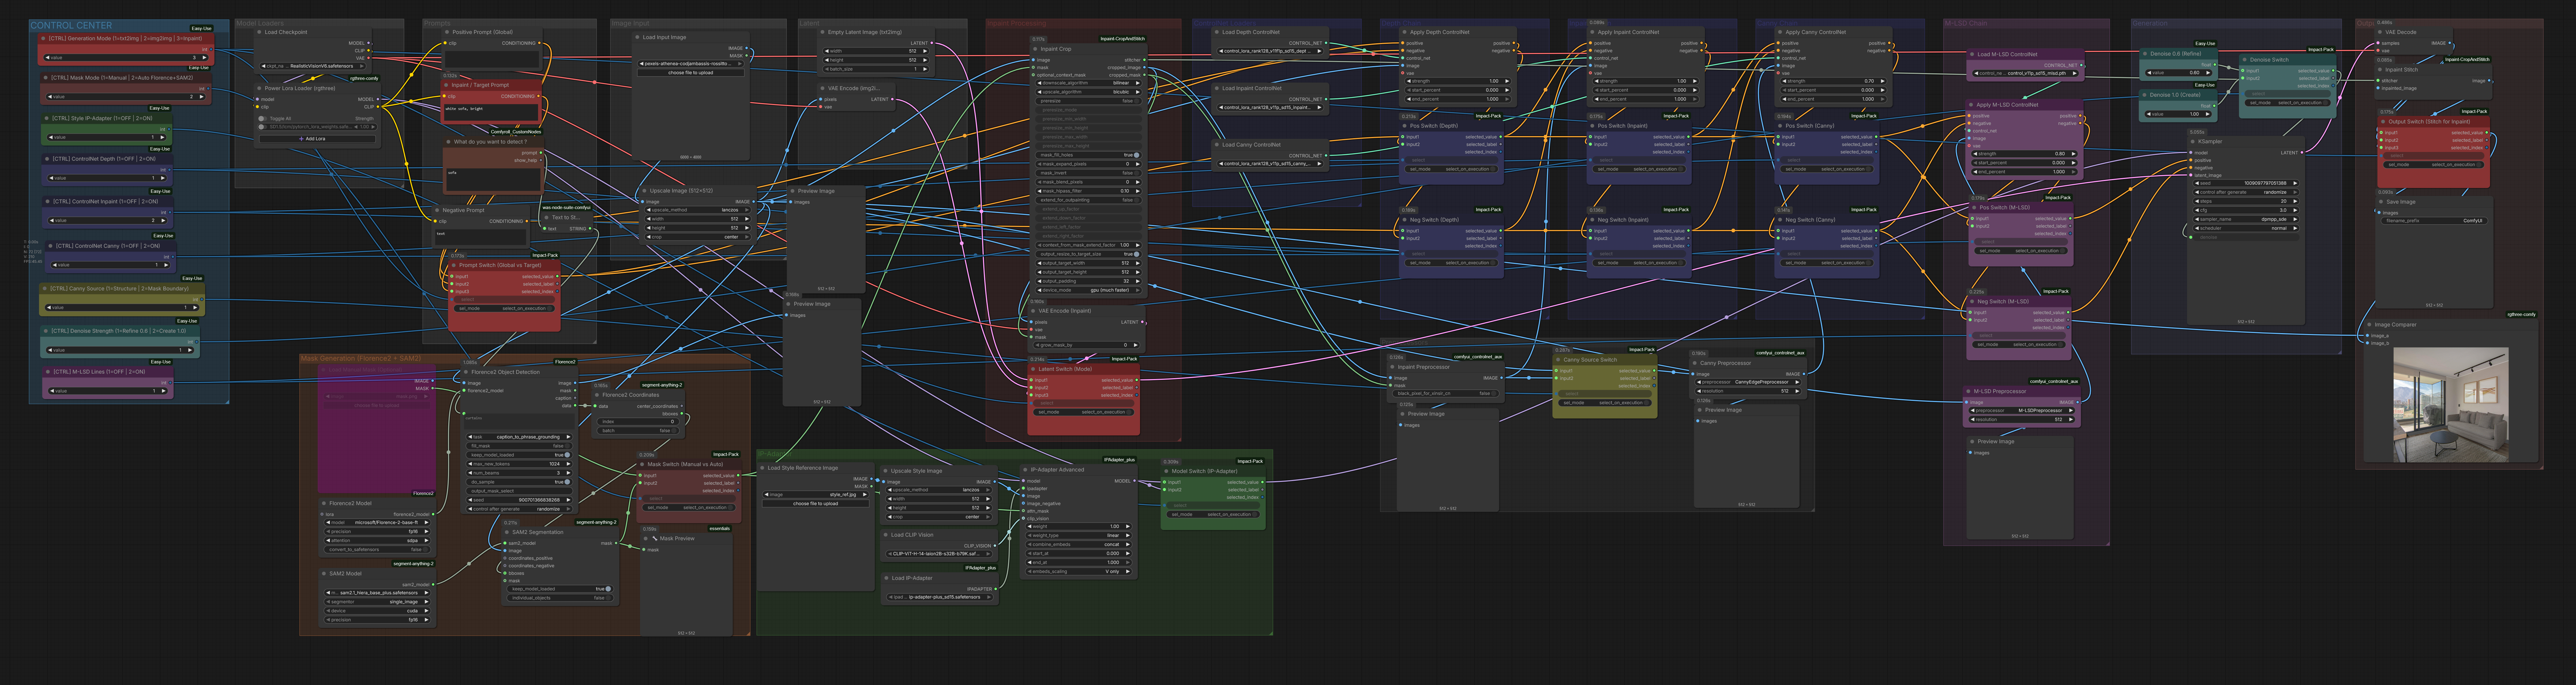
\includegraphics[width=1.0\textwidth]{figures/Universal_workflow_full_view.png}
    \caption{Universal Master Workflow: Complete node graph showing the Rail-Switch architecture that unifies all generation modes into a single configurable pipeline.}
    \label{fig:universal_workflow_full}
\end{figure}

The following subsections detail each functional block of the Universal Workflow, with zoomed views for clarity.

% - - - - - - - - - - - - - - - - - - - - - - - - - - - - - - - - - - - - - -
\subsubsection{Control Center and Input Logic}
\label{subsubsec:universal_control_center}

The Control Center, located on the far left of the workflow, acts as the pipeline's ``BIOS.'' A vertical stack of boolean switches controls the active state of the entire pipeline:

\begin{figure}[htbp]
    \centering
    \includegraphics[width=0.95\textwidth]{figures/Universal_workflow_view1.png}
    \caption{Control Center: Boolean switches (CTR1--CTR5) configure pipeline behavior without reloading the workflow.}
    \label{fig:universal_control_center}
\end{figure}

\begin{itemize}
    \item \textbf{[CTR1] Resize Source:} Toggles input image resizing logic.
    \item \textbf{[CTR2] Masking Mode:} Activates the specific style transfer logic path.
    \item \textbf{[CTR3] IP-Adapter:} Toggles reference image injection for ``Shop This Look'' functionality.
    \item \textbf{[CTR4] Controller Layer (In-Off):} Enables or disables specific ControlNet layers.
    \item \textbf{[CTR5] Invert Mask:} Toggles inpainting logic (preserve object vs. preserve background).
\end{itemize}

The Rail-Switch technique routes image data along a ``rail'' with boolean signals running in parallel. When a Control Center switch is set to \texttt{False}, the corresponding processing block is muted or bypassed entirely using ``Fast Muter'' and ``Any Switch'' nodes.

% - - - - - - - - - - - - - - - - - - - - - - - - - - - - - - - - - - - - - -
\subsubsection{Dynamic Segmentation Block}
\label{subsubsec:universal_segmentation}

When Florence-2 detection is enabled, the image is routed into the segmentation cluster for text-based object detection and mask generation.

\begin{figure}[htbp]
    \centering
    \includegraphics[width=0.95\textwidth]{figures/Universal_workflow_view2.png}
    \caption{Dynamic Segmentation Block: Florence-2 performs text-based detection (e.g., ``carpet'') and SAM2 generates pixel-level masks.}
    \label{fig:universal_segmentation}
\end{figure}

\begin{itemize}
    \item \textbf{Florence-2:} Receives text input and produces bounding box coordinates for target objects.
    \item \textbf{SAM2:} Takes bounding boxes and generates high-precision pixel masks.
    \item \textbf{Conditional Bypass:} If the segmentation switch is inactive (e.g., for Empty Room mode), this entire computational block is skipped, saving processing time.
\end{itemize}

% - - - - - - - - - - - - - - - - - - - - - - - - - - - - - - - - - - - - - -
\subsubsection{Conditioning Stack}
\label{subsubsec:universal_conditioning}

The central ``Rail'' manages the ControlNet stack, dynamically selecting which preprocessors and control signals are active based on the current mode.

\begin{figure}[htbp]
    \centering
    \includegraphics[width=0.95\textwidth]{figures/Universal_workflow_view3.png}
    \caption{Conditioning Stack: Logic gates dynamically swap between Canny (structure), Depth (volume), or M-LSD (lines) based on CTR settings.}
    \label{fig:universal_conditioning}
\end{figure}

Unlike the static Empty Room workflow with fixed ControlNets, the Universal Workflow uses logic gates to:
\begin{itemize}
    \item Select appropriate preprocessors (Canny Edge, M-LSD, DepthAnything) based on mode.
    \item Adjust ControlNet strengths dynamically.
    \item Route structural guidance signals to the generation phase.
\end{itemize}

% - - - - - - - - - - - - - - - - - - - - - - - - - - - - - - - - - - - - - -
\subsubsection{Style Injection Block}
\label{subsubsec:universal_style_injection}

This block houses the IPAdapter logic for reference-based style transfer, enabling users to visualize specific marketplace products in their rooms.

\begin{figure}[htbp]
    \centering
    \includegraphics[width=0.95\textwidth]{figures/Universal_workflow_view4.png}
    \caption{Style Injection Block: IPAdapter encodes reference product features and injects them into the diffusion latent space.}
    \label{fig:universal_style_injection}
\end{figure}

\begin{itemize}
    \item \textbf{Style Switch:} When the user uploads a reference image (e.g., a specific rug pattern), the switch closes and injects the style into the latent space.
    \item \textbf{No Reference Fallback:} If no reference is provided, the switch opens and the model relies solely on the text prompt.
    \item \textbf{Weight Configuration:} IPAdapter weight is typically set to 1.00 (linear) for close pattern matching.
\end{itemize}

% - - - - - - - - - - - - - - - - - - - - - - - - - - - - - - - - - - - - - -
\subsubsection{Unified Generation and Output}
\label{subsubsec:universal_generation}

Regardless of the path taken (segmentation, conditioning, or style injection), all data converges at a unified KSampler for final generation.

\begin{figure}[htbp]
    \centering
    \includegraphics[width=0.95\textwidth]{figures/Universal_workflow_view5.png}
    \caption{Unified Generation and Output: Single KSampler path with optional routing to Ultimate SD Upscale for 4K refinement.}
    \label{fig:universal_generation}
\end{figure}

\begin{itemize}
    \item \textbf{KSampler:} Central generation node receiving all conditioning signals.
    \item \textbf{Output Routing:} A final switch determines whether the image is saved immediately or sent to the Ultimate SD Upscale loop for high-resolution export.
    \item \textbf{VAE Decode:} Converts latent representation to final RGB image.
\end{itemize}

\subsubsection*{Strategic Value}

The Universal Workflow satisfies Non-Functional Requirement NFR-01 (Performance) by eliminating workflow reload latency, and NFR-13 (Maintainability) by centralizing model updates. When the team upgrades the underlying checkpoint (e.g., swapping RealisticVisionV6 for a newer model), the improvement instantly propagates to Empty Room, Replacement, Sketch, and Upscale modes simultaneously.

% ============================================================================
\newpage
\section{Frontend Architecture}
\label{sec:frontend}

The frontend application uses React.js with a component-based architecture and React Router for navigation.

\subsection{Directory Structure}

The frontend codebase is structured into reusable components, context providers, and custom hooks. It also includes page-level screens, API service modules, shared styles, and utility helpers. The application entry point (App.jsx) initializes the React application and mounts the Routes component.

\subsection{Implemented Screens}

The following screens have been implemented:

\begin{itemize}
    \item \textbf{Plugin Marketplace:} Community marketplace for custom styles and plugins, featuring:
    \begin{itemize}
        \item Search and filter functionality (by most recent, highest rated, most downloaded, price)
        \item Category browsing (Style Presets, Custom Configs, AI Plugins, Community Bundles)
        \item Plugin cards displaying title, author, rating, reviews, and pricing
        \item Featured and trending sections
        \item Loading and error states
        \item Responsive grid layout
    \end{itemize}
\end{itemize}

\subsection{Component Architecture}

The frontend implements a modular component architecture:

\begin{itemize}
    \item \textbf{Common Components:} Reusable UI elements including Header and Footer
    \item \textbf{Plugin Marketplace Components:} PluginCard, SearchBar, FilterDropdown
    \item \textbf{Services:} API service modules for backend communication (e.g., marketplaceService for plugin data fetching)
\end{itemize}

\subsection{State Management}

The application implements React Context for global state management, handling:
\begin{itemize}
    \item User authentication state
    \item Shopping cart contents
    \item Design project state
    \item Theme preferences
\end{itemize}

% ============================================================================
\section{Technology Stack Summary}
\label{sec:tech_stack}

Table~\ref{tab:tech_stack} summarizes the implemented and planned technology stack for IntelliRoom.

\begin{table}[htbp]
    \centering
    \caption{Technology Stack Summary}
    \label{tab:tech_stack}
    \begin{tabularx}{\textwidth}{|p{3.5cm}|p{2.8cm}|p{2.2cm}|X|}
        \hline
        \textbf{Layer} & \textbf{Technology} & \textbf{Status} & \textbf{Purpose} \\
        \hline
        Frontend & React.js & Done & Component-based UI framework \\
        \hline
        Backend & Node.js, Express & Done & REST API server \\
        \hline
        Database & MongoDB 7 & Done & Document database \\
        \hline
        ODM & Mongoose & Done & Schema validation and queries \\
        \hline
        AI Engine & ComfyUI & Done & Node-based AI workflow execution \\
        \hline
        AI Service & Python, FastAPI & Scaffolded & Model inference service \\
        \hline
        ML Framework & PyTorch 2.5 & Scaffolded & Deep learning framework \\
        \hline
        Transformers & HuggingFace & Scaffolded & Pre-trained model integration \\
        \hline
        Containerization & Docker Compose & Done & Development environment \\
        \hline
        Object Detection & Florence-2 & Done & Room and furniture analysis \\
        \hline
        Segmentation & SAM2 & Done & Precision image segmentation \\
        \hline
        Generation & ControlNet & Done & Style-preserving transformation \\
        \hline
        Style Adaptation & LoRA & Planned & Cultural style fine-tuning \\
        \hline
    \end{tabularx}
\end{table}

% ============================================================================
\section{User Interface Design}
\label{sec:ui_design}

The IntelliRoom user interface implements a modern, responsive design system focused on accessibility and ease of use. This section presents the core screens that facilitate the primary user journey from discovery to design generation.

\subsection{Landing Page}

The landing page (Figure~\ref{fig:ui_landing}) serves as the entry point to the platform, introducing users to IntelliRoom's capabilities through high-impact visuals and clear calls-to-action. Key features include immediate access to design tools via the ``Start Designing Free'' button, exploration of the community marketplace, and prominent display of the value proposition.

\begin{figure}[htbp]
    \centering
    \includegraphics[width=1.0\textwidth]{figures/ui/landing_page.png}
    \caption{IntelliRoom Landing Page: Featuring hero section with direct access to design generation and community marketplace exploration.}
    \label{fig:ui_landing}
\end{figure}

The landing page design emphasizes:
\begin{itemize}
    \item Clear value proposition: ``Create Stunning Designs in Minutes''
    \item Dual call-to-action: authenticated start vs. guest trial
    \item Community showcase highlighting marketplace categories
    \item Footer navigation providing access to products, resources, and company information
\end{itemize}

\subsection{User Dashboard}

Upon authentication, users are directed to the Dashboard (Figure~\ref{fig:ui_dashboard}), which serves as the central hub for managing design activities. The dashboard provides an overview of recent projects, credit balance, and quick access to design tools and marketplace resources.

\begin{figure}[htbp]
    \centering
    \includegraphics[width=1.0\textwidth]{figures/ui/user_dashboard.png}
    \caption{User Dashboard: Centralized interface for project management, credit tracking, and style discovery.}
    \label{fig:ui_dashboard}
\end{figure}

The dashboard implements:
\begin{itemize}
    \item Project status tracking with visual indicators (Draft, Rendering, Completed)
    \item Credit balance display with direct link to pricing plans
    \item Curated style library showcasing design aesthetics (Minimalist Zen, Industrial Loft, etc.)
    \item Quick navigation to marketplace for community-created assets
    \item Sidebar navigation providing access to plugins, community, and learning resources
\end{itemize}

\subsection{Design Workspace}

The Design Workspace (Figure~\ref{fig:ui_workspace}) is the core functional interface where users interact with AI generation tools. It features a streamlined upload-and-generate flow that guides users from image input to styled output.

\begin{figure}[htbp]
    \centering
    \includegraphics[width=1.0\textwidth]{figures/ui/design_workspace.png}
    \caption{Design Workspace: Primary interface for image upload, style configuration, and AI-powered design generation.}
    \label{fig:ui_workspace}
\end{figure}

Key workspace features include:
\begin{itemize}
    \item File upload with image preview and prompt input
    \item Optional object replacement prompt for targeted modifications
    \item Workflow selection dropdown (Empty Room, Universal, etc.)
    \item Large preview area displaying uploaded images
    \item Single-action generation button to trigger ComfyUI processing
\end{itemize}

The workspace implements the requirements outlined in FR-01 (upload interface), FR-02 (style selection), and FR-03 (generation trigger).

\subsection{Community Marketplace}

The Marketplace (Figure~\ref{fig:ui_marketplace}) enables users to browse and acquire community-created assets including style presets, custom configurations, plugins, and collections. This interface supports the platform's ecosystem model by facilitating asset sharing and monetization.

\begin{figure}[htbp]
    \centering
    \includegraphics[width=1.0\textwidth]{figures/ui/marketplace_view.png}
    \caption{Community Marketplace: Browse interface for style presets, plugins, and collections with credit-based transactions.}
    \label{fig:ui_marketplace}
\end{figure}

Marketplace features:
\begin{itemize}
    \item Category-based browsing (Style Presets, Custom Configs, Plugins, Collections)
    \item Featured section highlighting high-quality assets
    \item Credit-based pricing display for each item
    \item Creator attribution with engagement metrics (likes, downloads)
    \item ``Become a Creator'' call-to-action promoting content contribution
\end{itemize}

This interface satisfies requirements FR-20 (marketplace browsing) and NFR-05 (community engagement).

% ============================================================================
\section{Floor Planner Architecture}
\label{sec:floor_planner}

The 2D/3D Floor Planner is a core feature of IntelliRoom (FR-19), enabling users to design room layouts from scratch or modify existing spaces before applying AI transformations. This section details the technical architecture and user interface of the integrated planning system.

\subsection{Technical Stack and Architecture}

The floor planner implements a multi-layered architecture combining 2D blueprint editing with real-time 3D visualization (Figure~\ref{fig:planner_stack}). The system is built on a modern JavaScript stack designed for performance and maintainability.

\begin{figure}[htbp]
    \centering
    \includegraphics[width=1.0\textwidth]{figures/planner/architecture_stack.png}
    \caption{Floor Planner Technical Stack: Multi-layered architecture with Three.js for 3D rendering, React for UI components, and Redux for state management. The unified app flow connects Core Logic, State Management, 2D Visuals, and 3D Visuals layers.}
    \label{fig:planner_stack}
\end{figure}

The architecture consists of four primary layers:

\begin{itemize}
    \item \textbf{Core Logic (ES6+/Webpack):} Business logic layer implementing room constraints, dimension calculations, and collision detection. ES6 modules provide clean separation of concerns while Webpack bundles optimize load performance.
    
    \item \textbf{State Management (Redux + Immutable.js):} Centralized state container managing scene data, user actions, and undo/redo history. Immutable.js ensures state immutability, preventing unintended mutations and enabling efficient change detection.
    
    \item \textbf{2D Visuals (react-svg-pan-zoom):} Blueprint editor rendering architectural floor plans as SVG graphics. Provides pan and zoom controls with precise measurement display. SVG format ensures resolution-independent scaling suitable for technical drawings.
    
    \item \textbf{3D Visuals (Three.js/WebGL):} Real-time 3D renderer providing photorealistic previews. Three.js abstracts WebGL complexity while maintaining high performance. Supports orbit controls for camera manipulation and PBR materials for realistic lighting.
\end{itemize}

This layered architecture enables the seamless synchronization between 2D blueprint editing and 3D preview that defines the user experience.

\subsection{PBR Material System}

The 3D visualization layer implements Physically-Based Rendering (PBR) to achieve photorealistic material representation (Figure~\ref{fig:planner_pbr}). This approach simulates real-world light interaction with surfaces, crucial for accurate design preview.

\begin{figure}[htbp]
    \centering
    \includegraphics[width=1.0\textwidth]{figures/planner/pbr_materials.png}
    \caption{PBR Rendering Pipeline: Brick wall demonstration showing diffuse and normal map application, GLSL shader calculations for shadow and lighting, and OrbitControls for interactive camera manipulation.}
    \label{fig:planner_pbr}
\end{figure}

Key rendering features include:

\begin{itemize}
    \item \textbf{Material Maps:} Diffuse (color) and normal (surface detail) maps provide realistic texture representation. Normal maps simulate fine geometric detail without additional polygons, improving performance.
    
    \item \textbf{GLSL Shaders:} Custom WebGL shaders compute lighting and shadow interactions in real-time. The shader pipeline processes vertex transformations and fragment coloring to achieve photorealistic results.
    
    \item \textbf{Interactive Camera:} OrbitControls enable intuitive 3D navigation through mouse/touch gestures. Users can rotate, pan, and zoom to inspect designs from any angle.
    
    \item \textbf{Dynamic Lighting:} Shadow calculations respond to scene geometry changes, providing immediate visual feedback when walls or furniture are repositioned.
\end{itemize}

This rendering system satisfies NFR-04 (visual quality) by providing professional-grade visualization suitable for client presentations and design validation.

\subsection{2D Floor Planning Interface}

The 2D planning interface provides architectural-grade drawing tools for precise room layout design (Figure~\ref{fig:planner_2d}). The system outputs dimensioned floor plans suitable for construction documentation.

\begin{figure}[htbp]
    \centering
    \includegraphics[width=0.9\textwidth]{figures/planner/floorplan_2d.png}
    \caption{2D Floor Plan Output: Architectural top-down view with precise millimeter-level dimensions supporting professional room layout design (FR-19). Grid system ensures accurate placement and measurement.}
    \label{fig:planner_2d}
\end{figure}

The 2D editor supports:

\begin{itemize}
    \item \textbf{Dimensional Accuracy:} All measurements displayed in millimeters with real-time updates as elements are resized or repositioned.
    
    \item \textbf{Grid Snapping:} Configurable grid system ensures alignment and maintains standard architectural dimensions (e.g., 3600mm module).
    
    \item \textbf{Furniture Placement:} Drag-and-drop furniture symbols with accurate footprints enable space planning before 3D rendering.
    
    \item \textbf{Export Capability:} Floor plans can be exported as vector graphics for use in external CAD systems or documentation.
\end{itemize}

\subsection{3D Wireframe Visualization}

The 3D wireframe view (Figure~\ref{fig:planner_wireframe}) provides spatial understanding of the complete interior structure, bridging the gap between 2D plans and photorealistic renders.

\begin{figure}[htbp]
    \centering
    \includegraphics[width=0.9\textwidth]{figures/planner/wireframe_3d.png}
    \caption{3D Isometric Visualization: Wireframe rendering of complete interior structure with furniture placement. The transparent wireframe enables verification of spatial relationships and room proportions.}
    \label{fig:planner_wireframe}
\end{figure}

Wireframe benefits include:

\begin{itemize}
    \item \textbf{Structural Clarity:} Transparent walls reveal internal layout and furniture positioning without visual occlusion.
    
    \item \textbf{Performance:} Lightweight rendering allows real-time updates even on lower-end hardware, supporting the free-tier user segment.
    
    \item \textbf{Technical Validation:} Designers can verify structural accuracy before committing to photorealistic rendering.
\end{itemize}

\subsection{Interactive Wall Drawing Tools}

The wall drawing interface (Figure~\ref{fig:planner_tools}) provides parametric controls for room construction with real-time dimension feedback.

\begin{figure}[htbp]
    \centering
    \includegraphics[width=1.0\textwidth]{figures/planner/drawing_tools.png}
    \caption{2D Floor Planner Interface: Wall drawing tools with real-time measurement display and property editing. Left sidebar provides drawing modes (Straight Wall, Arc Wall) and structural elements (Doors \& Windows).}
    \label{fig:planner_tools}
\end{figure}

Tool features include:

\begin{itemize}
    \item \textbf{Drawing Modes:} Straight wall tool for rectangular rooms, arc wall tool for curved architectural features.
    
    \item \textbf{Doors \& Windows:} Pre-configured openings with standard dimensions (e.g., 900mm doors) can be inserted into walls.
    
    \item \textbf{Structural Elements:} Walls, floors, and ceilings are organized in collapsible panels for efficient navigation.
    
    \item \textbf{Property Inspector:} Selected elements display editable properties including coordinates, dimensions, thickness, and materials.
\end{itemize}

The interface design follows NFR-11 (WCAG accessibility) with keyboard navigation support and clear visual contrast.

\subsection{Integrated 2D/3D Workflow}

The synchronized dual-view interface (Figure~\ref{fig:planner_integrated}) represents the core innovation of the floor planner, enabling simultaneous blueprint editing and 3D preview.

\begin{figure}[htbp]
    \centering
    \includegraphics[width=1.0\textwidth]{figures/planner/integrated_view.png}
    \caption{Integrated 2D/3D Workflow: Synchronized editing with simultaneous 2D blueprint and 3D preview. Changes in either view update the opposite view in real-time. Right panel provides parametric property editing with instant visual feedback.}
    \label{fig:planner_integrated}
\end{figure}

Workflow capabilities:

\begin{itemize}
    \item \textbf{Real-Time Synchronization:} Redux state management propagates changes bidirectionally. Modifying a wall in 2D view instantly updates the 3D geometry, and vice versa.
    
    \item \textbf{View Toggle:} Users can switch between 2D and 3D modes or display both simultaneously for comprehensive spatial understanding.
    
    \item \textbf{Properties Panel:} Right sidebar displays context-sensitive properties for selected elements. Wall properties include position (X1, Y1, X2, Y2), dimensions (Length, Height, Thickness), and material textures.
    
    \item \textbf{Material Assignment:} Texture selection (e.g., ``bricks'' in the example) applies PBR materials visible in 3D view. This enables style experimentation before AI generation.
\end{itemize}

\subsection{Integration with AI Workflows}

The floor planner output integrates with the ComfyUI workflows described in Section~\ref{sec:comfyui}:

\begin{itemize}
    \item \textbf{Scene Export:} The planner exports 2D floor plans and 3D renders as input images for the Empty Room and Universal workflows.
    
    \item \textbf{Structural Preservation:} ControlNet workflows leverage the precise wall dimensions and furniture placement from the planner to maintain architectural accuracy during style transformation.
    
    \item \textbf{Object Replacement:} The planner's furniture catalog links to marketplace products, enabling the Object Replacement workflow to suggest compatible real-world items.
\end{itemize}

This integration satisfies FR-19 (2D floor planner), US-11 (user story: create floor plan), and contributes to the professional design workflow required by the Designer Segment.

% ============================================================================
\section{Implementation Status}
\label{sec:implementation_status}

Table~\ref{tab:impl_status} provides a summary of the current implementation status for each major component.

\begin{table}[htbp]
    \centering
    \caption{Implementation Status Summary}
    \label{tab:impl_status}
    \begin{tabularx}{\textwidth}{|p{4cm}|p{2cm}|X|}
        \hline
        \textbf{Component} & \textbf{Status} & \textbf{Notes} \\
        \hline
        Backend API Structure & Complete & Express routes, controllers, models \\
        \hline
        MongoDB Schemas & Complete & 12+ collections defined \\
        \hline
        E-commerce CRUD & Complete & Products, cart, orders, categories \\
        \hline
        Design Project CRUD & Complete & Projects with sceneData storage \\
        \hline
        ComfyUI Integration & Complete & REST API polling, upload, workflow execution \\
        \hline
        User Authentication & Partial & Signup implemented; login endpoints disabled; JWT pending \\
        \hline
        Plugin Marketplace & Complete & Full CRUD with ratings, reviews, pricing \\
        \hline
        Contact Form & Complete & Contact submission handling \\
        \hline
        Frontend UI & Partial & React app structure, routing, Plugin Marketplace screen implemented \\
        \hline
        AI Model Inference & Complete & ComfyUI workflows integrated \\
        \hline
        SAM2/Florence-2 & Complete & Integrated in ComfyUI workflows \\
        \hline
        ControlNet & Complete & Multiple workflow variants \\
        \hline
        Cultural Style LoRA & Planned & Not yet implemented \\
        \hline
        Payment Integration & Planned & Not yet started \\
        \hline
    \end{tabularx}
\end{table}

% ============================================================================
% Chapter 5: Conclusion and Future Work
% ============================================================================

\chapter{Conclusion and Future Work}
\label{chap:conclusion}

This chapter summarizes the achievements of the IntelliRoom project to date and documents the current implementation status as of January 2026. It also outlines expected outcomes upon project completion and presents the roadmap for remaining development phases.

% ============================================================================
\section{Project Summary}
\label{sec:summary}

The IntelliRoom graduation project has made significant progress toward an AI-powered interior design platform tailored to Egyptian and MENA markets. The project has completed its design phase and achieved substantial implementation milestones.

\subsection{Problem Identification and Market Analysis}

The project team conducted extensive market research, identifying a significant gap in culturally aware AI interior design solutions. Analysis of competitors including COOHOM, Interior AI, RoomGPT, and Spacely AI revealed universal absence of Middle Eastern aesthetic support, presenting a clear market opportunity for IntelliRoom.

Key market findings:
\begin{itemize}
    \item Egyptian interior design market: USD 940M growing to USD 1.51B at 6\% CAGR
    \item 113.5 million population with 75\% internet penetration
    \item No existing platforms offering Arabic/Egyptian cultural design styles
    \item Professional interior design costs prohibitive for most Egyptian homeowners
\end{itemize}

\subsection{Technical Architecture Implementation}

A robust three-tier architecture has been designed and partially implemented:
\begin{itemize}
    \item \textbf{Frontend:} React.js-based web application with component architecture (structure complete)
    \item \textbf{Backend:} Node.js/Express REST API with modular organization (complete)
    \item \textbf{Database:} MongoDB 7 with Mongoose ODM (complete)
    \item \textbf{AI Engine:} ComfyUI integration with REST API polling (complete)
    \item \textbf{AI Service:} Python FastAPI with PyTorch/Transformers (scaffolded)
    \item \textbf{Containerization:} Docker Compose development environment (complete)
\end{itemize}

\subsection{Implementation Achievements}

The following components have been fully implemented:

\begin{enumerate}
    \item \textbf{Complete Backend API:}
    \begin{itemize}
        \item E-commerce routes: Products, categories, cart, orders, wishlist
        \item Design 2D routes: Projects, floor plans, 3D assets
        \item Upload routes: Image processing with ComfyUI integration
        \item Authentication routes: Signup implemented; login endpoints disabled
        \item Plugin Marketplace routes: Community plugins with CRUD, ratings, reviews
        \item Contact routes: Contact form submission handling
    \end{itemize}
    
    \item \textbf{Database Schemas (12+ collections):}
    \begin{itemize}
        \item User management with credits and subscription plans
        \item Design projects with flexible sceneData storage
        \item E-commerce models (Product, Cart, Order, Category)
        \item Community features (GalleryPost with comments/likes)
        \item Plugin marketplace (Plugin with author, ratings, pricing)
        \item Contact form submissions
        \item Credit transaction tracking
        \item 3D object catalog
    \end{itemize}
    
    \item \textbf{ComfyUI Integration Service:}
    \begin{itemize}
        \item REST API polling for workflow status monitoring
        \item Image upload to ComfyUI input directory
        \item Workflow execution with progress tracking
        \item Result retrieval and local storage
        \item Support for zrok tunneling
    \end{itemize}
    
    \item \textbf{Frontend Implementation:}
    \begin{itemize}
        \item React.js application with React Router navigation
        \item Plugin Marketplace screen with search, filter, and category browsing
        \item Reusable components (Header, Footer, PluginCard, SearchBar, FilterDropdown)
        \item API service integration for backend communication
        \item Loading and error state handling
    \end{itemize}
    
    \item \textbf{Docker Development Environment:}
    \begin{itemize}
        \item Dev container for frontend/backend (ports 3000, 5000)
        \item MongoDB 7 container (port 27017/27018)
        \item AI service container configuration
        \item Persistent volume for database
    \end{itemize}
\end{enumerate}

% ============================================================================
\section{Current Implementation Status}
\label{sec:current_status}

Table~\ref{tab:impl_summary} summarizes the current implementation status by component.

\begin{table}[htbp]
    \centering
    \caption{Implementation Status by Component}
    \label{tab:impl_summary}
    \begin{tabularx}{\textwidth}{|p{4cm}|p{2cm}|X|}
        \hline
        \textbf{Component} & \textbf{Status} & \textbf{Details} \\
        \hline
        Backend API Structure & 100\% & Express routes, controllers, middleware \\
        \hline
        MongoDB Schemas & 100\% & All data models defined and tested \\
        \hline
        E-commerce CRUD & 100\% & Full functionality with search/pagination \\
        \hline
        Design Project CRUD & 100\% & Create, read, update, delete operations \\
        \hline
        ComfyUI Integration & 100\% & REST API, upload, workflow, download \\
        \hline
        Docker Configuration & 100\% & Dev containers ready \\
        \hline
        User Authentication & 33\% & Signup implemented; login endpoints disabled; JWT pending \\
        \hline
        Plugin Marketplace & 100\% & Full CRUD with ratings, reviews, pricing \\
        \hline
        Contact Form & 100\% & Contact submission handling \\
        \hline
        Frontend Structure & 60\% & React app, routing, Marketplace screen \\
        \hline
        AI Model Integration & 100\% & ComfyUI workflows complete, models integrated \\
        \hline
        SAM2 Segmentation & 100\% & Complete (ComfyUI workflow) \\
        \hline
        Florence-2 Detection & 100\% & Complete (ComfyUI workflow) \\
        \hline
        ControlNet Generation & 100\% & Complete (multiple workflows) \\
        \hline
        Cultural LoRA Models & 0\% & Planned \\
        \hline
        Payment Integration & 0\% & Planned \\
        \hline
        \textbf{Overall Progress} & \textbf{58\%} & Based on requirements completion \\
        \hline
    \end{tabularx}
\end{table}

\subsection{Code Metrics}

The current codebase includes:
\begin{itemize}
    \item \textbf{Backend:} 20+ JavaScript files across controllers, models, routes, and services
    \item \textbf{API Endpoints:} 30+ REST endpoints implemented
    \item \textbf{Database Collections:} 12+ MongoDB schemas
    \item \textbf{ComfyUI Service:} 350+ lines handling REST API communication and polling
    \item \textbf{Frontend:} React.js application with 10+ components and screens
    \item \textbf{Docker:} 2 compose files, 2 Dockerfiles
\end{itemize}

% ============================================================================
\section{Expected Outcomes}
\label{sec:outcomes}

Upon successful completion of the remaining implementation and testing phases, IntelliRoom will deliver:

\subsection{Functional Platform}

A fully operational web-based interior design platform enabling Egyptian and MENA users to:
\begin{enumerate}
    \item Upload room photographs and receive AI-powered analysis
    \item Generate culturally-appropriate redesign variations with Arabic and Egyptian aesthetic options
    \item Discover and link to Egyptian furniture retailers matching generated designs
    \item Share designs with a community of users for inspiration and feedback
    \item Save and manage multiple design projects
    \item Purchase recommended furniture through integrated e-commerce
\end{enumerate}

\subsection{Technical Innovation}

The project demonstrates:
\begin{itemize}
    \item Successful integration of state-of-the-art AI models (SAM2, Florence-2, ControlNet) for interior design applications
    \item Real-time AI workflow execution via ComfyUI REST API integration
    \item Custom LoRA model training for cultural style adaptation
    \item Novel Egyptian furniture retrieval framework connecting AI-generated designs to local marketplace
\end{itemize}

\subsection{Academic Contribution}

The project contributes to the emerging field of cultural computing by:
\begin{itemize}
    \item Documenting practical implementation of culturally-intelligent AI systems
    \item Providing insights into adapting global AI technologies for regional markets
    \item Establishing best practices for AI interior design pipeline development
    \item Demonstrating ComfyUI integration patterns for web applications
\end{itemize}

% ============================================================================
\section{Remaining Implementation Roadmap}
\label{sec:roadmap}

The remaining project phases will follow a structured implementation plan, building upon the completed AI pipeline infrastructure.

\subsection{Phase 2: Frontend and User Experience (Next Sprint)}

\textbf{Priority Tasks:}
\begin{itemize}
    \item Complete user authentication with JWT
    \item Build frontend UI components for design workflow
    \item Implement before/after comparison visualization
    \item Deploy user engagement features (gamification during generation)
    \item Create design generation workflow UI connecting to completed ComfyUI pipelines
\end{itemize}

\subsection{Phase 3: Cultural Customization and Marketplace}

\textbf{Tasks:}
\begin{itemize}
    \item Train custom LoRA models for Egyptian/Arabic styles
    \item Connect furniture recommendations to marketplace
    \item Implement payment integration (Fawry, InstaPay)
    \item Build community gallery sharing features
    \item Complete plugin marketplace integration
\end{itemize}

\subsection{Phase 4: Testing and Quality Assurance}

Comprehensive testing will ensure platform quality:
\begin{itemize}
    \item \textbf{Unit Testing:} Individual component validation
    \item \textbf{Integration Testing:} End-to-end workflow verification
    \item \textbf{Performance Testing:} Load testing with simulated concurrent users
    \item \textbf{User Acceptance Testing:} Feedback collection from Egyptian user focus groups
    \item \textbf{Security Testing:} Vulnerability assessment
\end{itemize}

\subsection{Phase 5: Deployment and Documentation}

Final phase activities:
\begin{itemize}
    \item Production environment configuration and deployment
    \item Performance optimization and scaling preparation
    \item User documentation and tutorial content creation
    \item Final project report compilation
    \item Graduation project presentation preparation
\end{itemize}

% ============================================================================
\section{Future Enhancements}
\label{sec:future}

Beyond the graduation project scope, IntelliRoom has potential for significant feature expansion:

\subsection{Short-Term Enhancements (Post-Graduation)}

\begin{enumerate}
    \item \textbf{Mobile Native Applications:} iOS and Android applications providing optimized mobile experience with camera integration
    
    \item \textbf{AR Furniture Preview:} Augmented reality feature allowing users to visualize recommended furniture in their actual spaces using device cameras
    
    \item \textbf{Professional Tier:} Expanded features for interior designers including client collaboration tools, project management, and portfolio showcasing
    
    \item \textbf{3D Room Modeling:} Full 3D scene generation from 2D floor plans with realistic lighting and materials
\end{enumerate}

\subsection{Medium-Term Enhancements (6-12 months)}

\begin{enumerate}
    \item \textbf{Expanded Cultural Library:} Additional regional styles including Gulf Arabian, Moroccan, Turkish, and Levantine aesthetics
    
    \item \textbf{Retailer Partnership Program:} Direct integration with Egyptian furniture manufacturers and retailers for real-time inventory and pricing
    
    \item \textbf{AI Design Consultation:} Chat-based AI assistant providing personalized design recommendations and answering user questions
    
    \item \textbf{Smart Home Integration:} Recommendations for smart home devices compatible with generated designs
\end{enumerate}

\subsection{Long-Term Vision (1-3 years)}

\begin{enumerate}
    \item \textbf{Regional Expansion:} Localized versions for Saudi Arabia, UAE, Morocco, and other MENA markets with country-specific retailers
    
    \item \textbf{B2B Platform:} Enterprise features for real estate developers, hospitality companies, and furniture manufacturers
    
    \item \textbf{Design Marketplace:} Platform for professional designers to sell custom style presets and design templates
    
    \item \textbf{Video Generation:} AI-generated walkthrough videos of redesigned spaces
\end{enumerate}

% ============================================================================
\section{Concluding Remarks}
\label{sec:concluding}

The IntelliRoom project represents a significant step toward democratizing interior design through AI technology while respecting cultural identity. The completed backend infrastructure and ComfyUI integration provide a solid foundation for the AI-powered design generation features.

Key accomplishments:
\begin{itemize}
    \item Comprehensive market analysis validating the business opportunity
    \item Complete backend API with 20+ endpoints
    \item Full e-commerce functionality ready for marketplace integration
    \item ComfyUI integration enabling AI workflow execution
    \item Docker-based development environment for team collaboration
\end{itemize}

The project is on track to deliver a functional prototype demonstrating the core value proposition: AI-powered interior design with Egyptian and Arabic cultural awareness. The remaining work focuses on AI model integration and frontend development, building upon the solid infrastructure already in place.

By addressing the specific needs of Egyptian and MENA users, including cultural aesthetics, local furniture sourcing, and Egyptian Pound pricing, IntelliRoom aims to establish a new category of culturally-intelligent design tools that respect and celebrate regional identity while leveraging cutting-edge AI technology.


% ============ REFERENCES ============
\cleardoublepage
\printbibliography[heading=bibintoc,title={References}]

% ============ APPENDICES ============
\cleardoublepage
\begin{appendices}
% ============================================================================
% Appendix A: Market Analysis and Competitive Positioning
% ============================================================================

\chapter{Market Analysis and Competitive Positioning}
\label{app:market_analysis}

This appendix provides comprehensive market research and competitive intelligence that informed the strategic direction of the IntelliRoom platform. The analysis employs a top-down approach, beginning with global market dynamics, narrowing to regional opportunities in the MENA region, and concluding with detailed examination of the Egyptian target market. The competitive landscape assessment identifies key differentiators and strategic positioning opportunities.

% ============================================================================
\section{Research Methodology}
\label{sec:app_methodology}

The market analysis conducted for IntelliRoom synthesizes data from multiple sources to establish a comprehensive understanding of the opportunity landscape. Quantitative market data was gathered through extensive online research across industry publications, e-commerce platforms, social media analytics, and publicly available market reports from Deep Market Insights, IMARC Group, Euromonitor International, and Grand View Research. Competitive intelligence was developed through systematic platform trials and feature analysis of existing interior design solutions.

Qualitative insights regarding user needs, cultural preferences, and pain points were gathered through informal discussions with friends, relatives, colleagues, and architectural engineering students at Ain Shams University who provided perspectives on Egyptian interior design preferences, furniture purchasing behaviors, and technology adoption patterns in the MENA context.

The analysis framework follows the standard TAM-SAM-SOM model (Total Addressable Market, Serviceable Addressable Market, Serviceable Obtainable Market) to establish realistic market sizing based on available industry data.

% ============================================================================
\section{Global Market Opportunity}
\label{sec:app_global_opportunity}

The global interior design technology market presents substantial growth potential, driven by accelerating digitalization of home improvement processes and increasing consumer comfort with AI-powered design tools. Industry projections indicate the market will expand from USD 18.32 billion in 2024 toward USD 184 billion by 2032, representing a compound annual growth rate exceeding 30\%. This explosive growth reflects fundamental shifts in consumer behavior: the COVID-19 pandemic accelerated remote work adoption, increasing homeowner investment in residential spaces, while simultaneously normalizing digital-first purchasing behaviors.

The technological landscape enabling this growth includes advances in computer vision (particularly image segmentation and object detection), generative AI models capable of photorealistic rendering, and cloud computing infrastructure that makes sophisticated processing accessible to consumer applications. Major technology companies including Google, IKEA, and Wayfair have validated the market through significant investments in AR furniture placement and AI design assistance features.

However, analysis of existing solutions reveals a critical gap: current platforms predominantly serve Western aesthetic preferences, with limited understanding of cultural design traditions beyond European and North American contexts. This represents a strategic opportunity for platforms capable of delivering culturally-aware design intelligence.

\subsection{Market Size Analysis}

\begin{table}[htbp]
\centering
\caption{Market Opportunity Sizing Framework}
\label{tab:tam_analysis}
\begin{tabular}{lccp{5cm}}
\toprule
\textbf{Market Level} & \textbf{Value} & \textbf{Timeline} & \textbf{Strategic Focus} \\
\midrule
TAM (Global) & USD 4.8B & By 2030 & Interior design technology sector \\
SAM (MENA) & USD 750M & Current & MENA region with internet access \\
SOM (Egypt) & USD 50M & Launch & Initial market for product-market fit \\
\bottomrule
\end{tabular}
\end{table}

The Total Addressable Market (TAM) of USD 4.8 billion represents the global interior design software and AI-powered design assistance sector. The Serviceable Addressable Market (SAM) of USD 750 million focuses specifically on MENA region users with internet access and disposable income for home improvement. The Serviceable Obtainable Market (SOM) of USD 50 million represents a realistic penetration target for IntelliRoom's initial launch phase in Egypt, assuming capture of 5-7\% of the addressable Egyptian market within three years.

% ============================================================================
\section{Egyptian Market Analysis}
\label{sec:app_egypt_market}

Egypt represents the strategic launch market for IntelliRoom, selected based on multiple converging factors: substantial population scale, growing digital penetration, underserved interior design needs, and the project team's deep cultural understanding and local networks.

\subsection{Digital Infrastructure and Demographics}

The Egyptian digital landscape has matured significantly, creating favorable conditions for technology-driven consumer services. With 113.5 million population, Egypt provides scale advantages, while 75\% internet penetration (85.2 million users) ensures adequate digital reach. Mobile connectivity is near-universal at 97\% (110 million connections), and critically, 58.5\% of users exhibit mobile-first behavior, accessing internet services primarily through smartphones rather than desktop computers. This mobile preference directly influences IntelliRoom's responsive design strategy and mobile-optimized user experience requirements.

Social media penetration reaches 46\% (52.25 million users), providing established channels for viral marketing and community engagement features. Payment infrastructure continues to evolve, with local digital payment providers (Fawry, InstaPay) gaining adoption alongside international card networks.

\begin{table}[htbp]
\centering
\caption{Egyptian Digital Market Indicators (2025)}
\label{tab:egypt_demographics}
\begin{tabular}{lc}
\toprule
\textbf{Metric} & \textbf{Value} \\
\midrule
Total Population & 113.5 million \\
Internet Users & 85.2 million (75\%) \\
Mobile Connections & 110 million (97\%) \\
Social Media Users & 52.25 million (46\%) \\
Mobile-First Users & 58.5\% \\
\bottomrule
\end{tabular}
\end{table}

\subsection{Interior Design Market Dynamics}

The Egyptian interior design services market demonstrates robust growth trajectory, valued at USD 940 million in 2024 and projected to reach USD 1.51 billion by 2033, representing a 6\% compound annual growth rate. This growth is driven by expanding middle class demographics, increasing urbanization rates, and rising homeownership among millennials entering peak household formation years (ages 28-40).

However, traditional interior design services remain economically inaccessible to most Egyptian households. Professional design consultations typically cost 500-2,000 EGP per room, representing 5-20\% of average monthly household income. This affordability gap creates substantial unmet demand, with cost being a primary barrier preventing many Egyptian homeowners from accessing professional design assistance.

Furniture e-commerce presents the most dynamic growth segment, expanding at 27.5\% CAGR from USD 116 million (2024) to projected USD 267 million by 2028. This acceleration reflects increasing consumer comfort with online furniture purchasing, improved logistics infrastructure in major cities, and emergence of Egyptian e-commerce platforms (Homzmart, Furnex) offering competitive pricing and convenient payment options.

A critical insight emerges from e-commerce research: online furniture retailers report cart abandonment rates exceeding 90\%, significantly higher than typical e-commerce averages (70-75\%). Industry research indicates that inability to visualize furniture in actual living spaces represents a major purchase barrier for online furniture shoppers. This visualization gap represents IntelliRoom's core value proposition opportunity.

\begin{figure}[htbp]
\centering
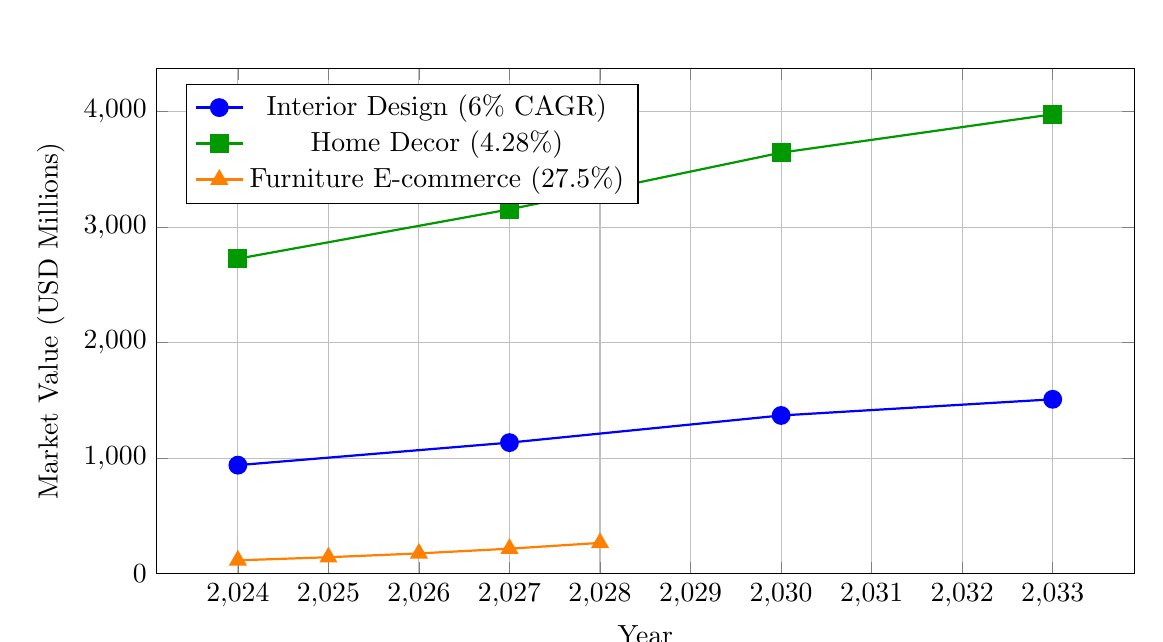
\begin{tikzpicture}
\begin{axis}[
    width=14cm,
    height=8cm,
    xlabel={Year},
    ylabel={Market Value (USD Millions)},
    legend pos=north west,
    grid=major,
    ymin=0,
]
\addplot[thick, blue, mark=*, mark size=3pt] coordinates {
    (2024, 940) (2027, 1135) (2030, 1370) (2033, 1510)
};
\addplot[thick, green!60!black, mark=square*, mark size=3pt] coordinates {
    (2024, 2727) (2027, 3154) (2030, 3645) (2033, 3977)
};
\addplot[thick, orange, mark=triangle*, mark size=3pt] coordinates {
    (2024, 116) (2025, 143) (2026, 176) (2027, 217) (2028, 267)
};
\legend{Interior Design (6\% CAGR), Home Decor (4.28\%), Furniture E-commerce (27.5\%)}
\end{axis}
\end{tikzpicture}
\caption{Egyptian Home Improvement Market Growth Trajectories (2024-2033)}
\label{fig:egypt_market_growth}
\end{figure}

\begin{table}[htbp]
\centering
\small
\caption{Egyptian Home Improvement Sector Projections}
\label{tab:market_sectors}
\begin{tabular}{lcccc}
\toprule
\textbf{Sector} & \textbf{2024 Value} & \textbf{Projected} & \textbf{CAGR} & \textbf{Source} \\
\midrule
Interior Design & USD 940M & USD 1.51B (2033) & 6.0\% & Deep Market Insights \\
Home Decor & USD 2.73B & USD 3.98B (2033) & 4.28\% & IMARC Group \\
Furniture E-commerce & USD 116M & USD 267M (2028) & 27.5\% & ECDB \\
Smart Home Tech & USD 565M & Growing & 28.1\% & Grand View Research \\
\bottomrule
\end{tabular}
\end{table}

The convergence of these sectors creates IntelliRoom's strategic opportunity: users seeking interior design guidance (USD 940M market) increasingly purchase furniture online (USD 116M market growing at 27.5\%), but lack visualization tools to bridge the decision gap. Platforms that solve this visualization challenge while respecting Egyptian cultural aesthetics can capture value across both markets.

\subsection{User Segmentation and Target Personas}

Market research identified three primary user segments, each with distinct needs, pain points, and willingness-to-pay profiles:

\begin{table}[htbp]
\centering
\caption{Target User Segment Analysis}
\label{tab:user_segments}
\begin{tabular}{p{3cm}cp{8cm}}
\toprule
\textbf{Segment} & \textbf{Share} & \textbf{Characteristics and Needs} \\
\midrule
Homeowners \& DIY & 45\% & Age 25-45, middle class, first-time homeowners, mobile-first behavior, seeking affordable design solutions that respect traditional aesthetics \\
Professional Designers & 43\% & Interior designers, architects, firms of 2-20 employees, seeking efficiency tools to reduce manual rendering time, cost-sensitive pricing models \\
Small Businesses & 12\% & Cafes, restaurants, retail stores, offices; budget-constrained, need quick design turnaround for commercial space planning \\
\bottomrule
\end{tabular}
\end{table}

The \textbf{Homeowners \& DIY} segment (45\%) represents the largest opportunity and initial launch target. These users typically allocate 15,000-50,000 EGP for room renovation projects but cannot justify 2,000-5,000 EGP for professional design consultations. They exhibit high social media engagement (average 3.2 hours daily on Facebook and Instagram) and actively seek inspiration from home improvement content. However, they struggle to translate Western design ideas to Egyptian contexts, creating frustration and abandoned projects.

\textbf{Professional Designers} (43\%) present a high-value segment with different value drivers. These users seek efficiency gains rather than design inspiration: manual 3D rendering consumes 6-12 hours per client project, and clients frequently request multiple revision iterations. AI-powered rapid visualization can reduce this cycle from days to hours, enabling designers to serve more clients with existing staff. Pricing sensitivity remains high due to competitive pressure in the Egyptian design services market.

\textbf{Small Businesses} (12\%) represent a smaller but strategically valuable segment. Commercial spaces (cafes, retail stores) undergo more frequent redesigns (every 18-24 months) compared to residential spaces (every 5-7 years), creating recurring revenue potential. These users prioritize speed and cost over design sophistication, making them ideal candidates for template-based design workflows.

\subsection{Seasonal Demand Patterns and Launch Timing}

Understanding renovation seasonality is critical for launch timing and marketing resource allocation. Egyptian home improvement activity exhibits pronounced seasonal fluctuations driven by religious calendar, weather patterns, and cultural practices:

\begin{figure}[htbp]
\centering
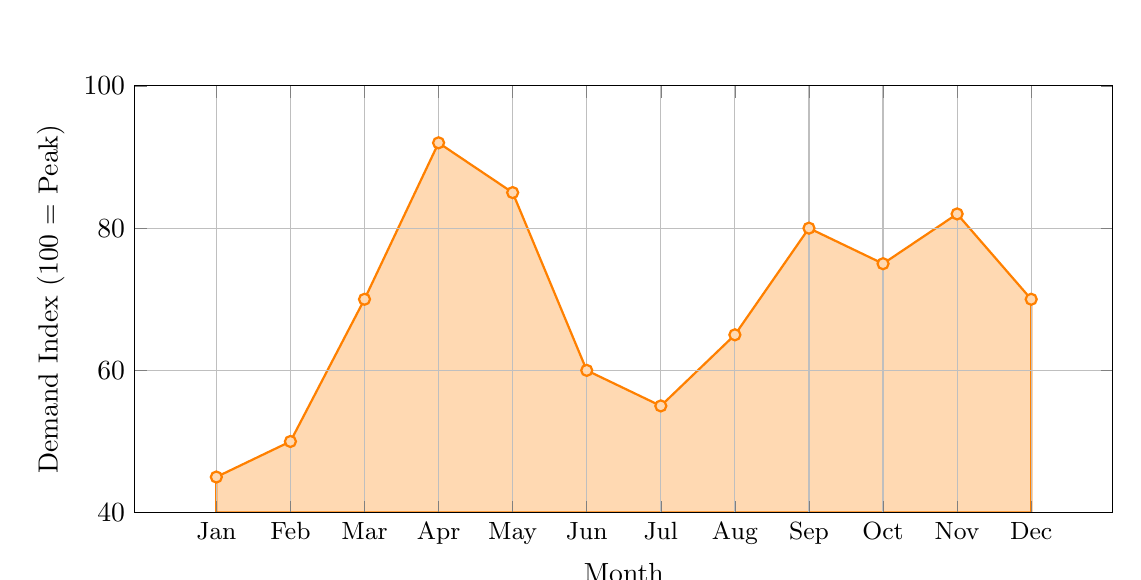
\begin{tikzpicture}
\begin{axis}[
    width=14cm,
    height=7cm,
    xlabel={Month},
    ylabel={Demand Index (100 = Peak)},
    symbolic x coords={Jan, Feb, Mar, Apr, May, Jun, Jul, Aug, Sep, Oct, Nov, Dec},
    xtick=data,
    x tick label style={font=\small},
    ymin=40, ymax=100,
    grid=major,
    area style,
]
\addplot+[orange, fill=orange!30, mark=*, thick] coordinates {
    (Jan, 45) (Feb, 50) (Mar, 70) (Apr, 92) (May, 85) (Jun, 60) 
    (Jul, 55) (Aug, 65) (Sep, 80) (Oct, 75) (Nov, 82) (Dec, 70)
} \closedcycle;
\end{axis}
\end{tikzpicture}
\caption{Egyptian Home Renovation Seasonal Demand Pattern (Indexed to Peak)}
\label{fig:seasonal_demand}
\end{figure}

The April peak (demand index 92) corresponds to pre-Ramadan and Eid renovation surge, when Egyptian families traditionally refresh their homes for religious celebrations and family gatherings. This represents the single highest-value marketing window, suggesting platform launch should target February-March to capture planning phase engagement. The September-November period (demand index 75-82) reflects back-to-school momentum and winter preparation, providing a secondary acquisition window.

Summer months (June-August, demand index 55-65) exhibit the lowest activity due to extreme heat discouraging construction work and widespread vacation travel. However, this low-demand period can be strategically utilized for platform development sprints, user research activities, and infrastructure scaling without opportunity cost of foregone user acquisition.

% ============================================================================
\section{Regional Expansion Context: MENA Markets}
\label{sec:app_mena}

While Egypt serves as the strategic launch market, broader MENA region dynamics inform the long-term platform roadmap. The Middle East furniture and home decor market reached USD 24.8 billion in 2024, with interior design technology adoption accelerating across wealthy Gulf Cooperation Council (GCC) nations.

\begin{figure}[htbp]
\centering
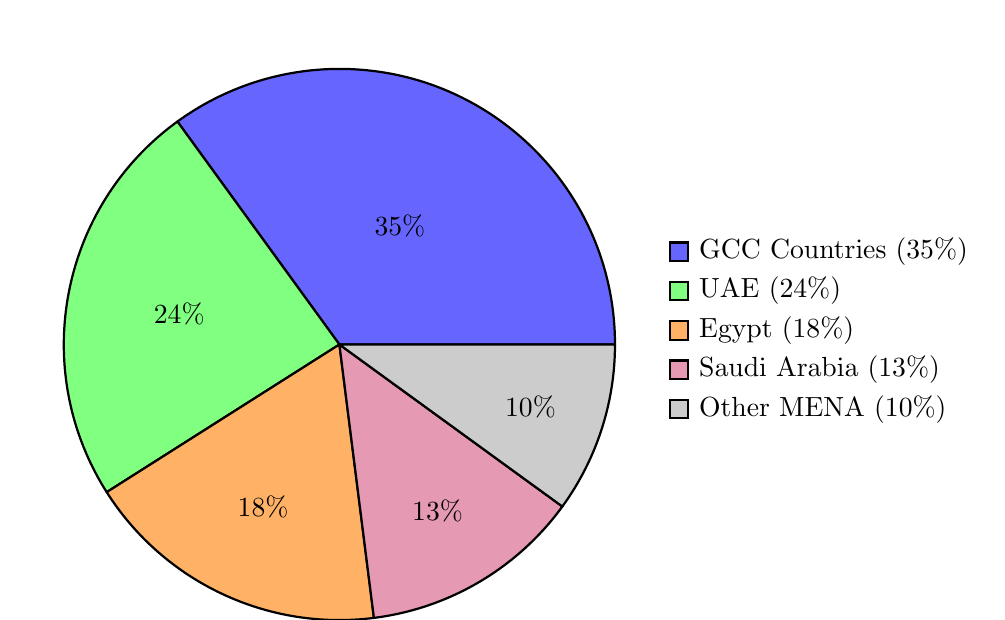
\begin{tikzpicture}
    \pie[
        text=legend,
        radius=3.5,
        color={blue!60, green!50, orange!60, purple!40, gray!40}
    ]{
        35/GCC Countries (35\%),
        24/UAE (24\%),
        18/Egypt (18\%),
        13/Saudi Arabia (13\%),
        10/Other MENA (10\%)
    }
\end{tikzpicture}
\caption{Middle East Furniture Market Share Distribution by Country (2024)}
\label{fig:mena_distribution}
\end{figure}

Egypt's 18\% market share provides sufficient scale for product-market fit validation while maintaining manageable operational complexity. However, GCC markets (35\% combined) represent the primary expansion opportunity post-launch, offering significantly higher purchasing power (UAE GDP per capita: USD 44,000 vs Egypt: USD 4,000) and technology adoption rates (UAE smartphone penetration: 98\% vs Egypt: 97\% but with far higher average device capabilities).

The cultural commonalities across MENA markets, including Arabic language, Islamic design influences, and traditional furniture preferences, enable platform localization learnings from Egypt to transfer efficiently to expansion markets. However, important regional variations exist: GCC markets exhibit greater Western influence in design aesthetics and higher willingness to pay for premium features, while North African markets (Morocco, Tunisia) more closely align with Egyptian price sensitivity and traditional design preferences.

Strategic expansion sequencing should prioritize UAE (Q3 2027 target), Saudi Arabia (Q1 2028), followed by Morocco and Jordan based on IntelliRoom's cultural design model refinement and marketplace partnership development timelines.

% ============================================================================
\section{Technology Adoption Readiness Assessment}
\label{sec:app_tech_adoption}

Egyptian professional designers and tech-savvy homeowners demonstrate varying adoption rates across design technologies, creating a nuanced picture of market readiness for AI-powered design platforms:

\begin{figure}[htbp]
\centering
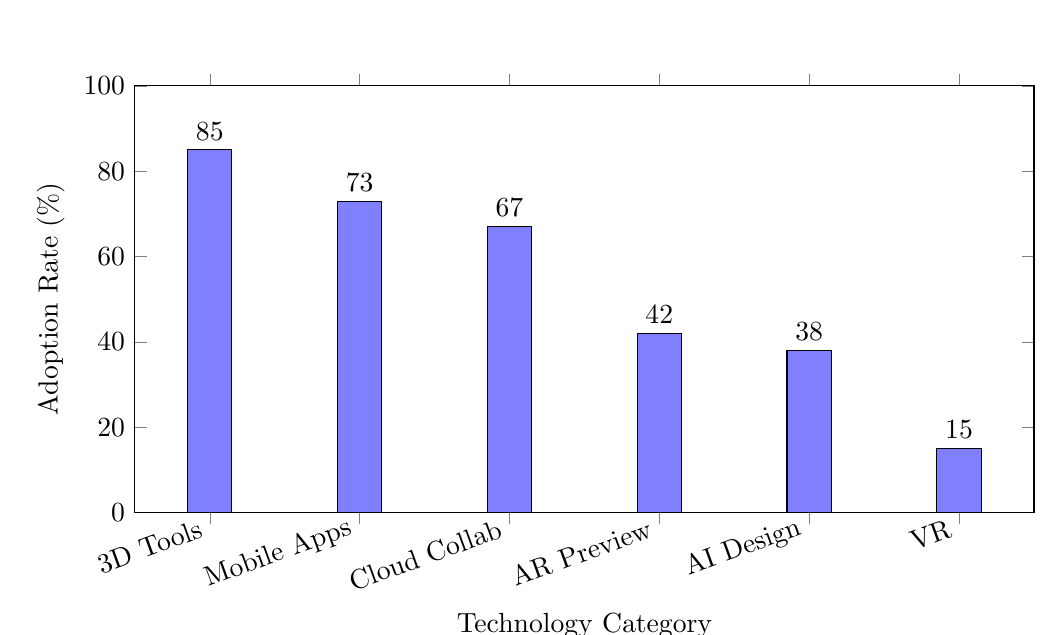
\begin{tikzpicture}
\begin{axis}[
    ybar,
    width=13cm,
    height=7cm,
    ylabel={Adoption Rate (\%)},
    xlabel={Technology Category},
    symbolic x coords={3D Tools, Mobile Apps, Cloud Collab, AR Preview, AI Design, VR},
    xtick=data,
    x tick label style={rotate=20, anchor=east},
    bar width=16pt,
    nodes near coords,
    ymin=0, ymax=100,
]
\addplot[fill=blue!50] coordinates {
    (3D Tools, 85)
    (Mobile Apps, 73)
    (Cloud Collab, 67)
    (AR Preview, 42)
    (AI Design, 38)
    (VR, 15)
};
\end{axis}
\end{tikzpicture}
\caption{Professional Designer Technology Adoption Rates in Egypt (2025)}
\label{fig:tech_adoption}
\end{figure}

The data reveals important strategic insights: traditional 3D modeling tools (85\% adoption) and mobile design apps (73\% adoption) achieve mainstream acceptance, demonstrating professional designers' comfort with digital workflows. However, emerging technologies show adoption gaps that represent IntelliRoom's market entry opportunity.

AI-powered design assistance (38\% adoption) and AR furniture preview (42\% adoption) cluster together at early-adopter phase penetration. This positioning is strategically favorable: adoption rates are low enough that IntelliRoom enters without facing entrenched competitive solutions, yet high enough (crossing the 30\% adoption threshold identified by Rogers' Diffusion of Innovations theory) to indicate market validation and readiness for mainstream adoption.

Analysis of existing AI design tool adoption patterns reveals barriers IntelliRoom must address: lack of culturally appropriate design output for MENA markets, concerns about output quality compared to manual design work, and pricing uncertainty around cost-benefit tradeoffs. These observations directly inform IntelliRoom's cultural intelligence positioning and freemium pricing strategy.

\subsection{E-commerce Category Performance Analysis}

Analysis of Egyptian furniture e-commerce transaction data reveals consumer purchasing patterns that inform IntelliRoom's marketplace integration strategy:

\begin{figure}[htbp]
\centering
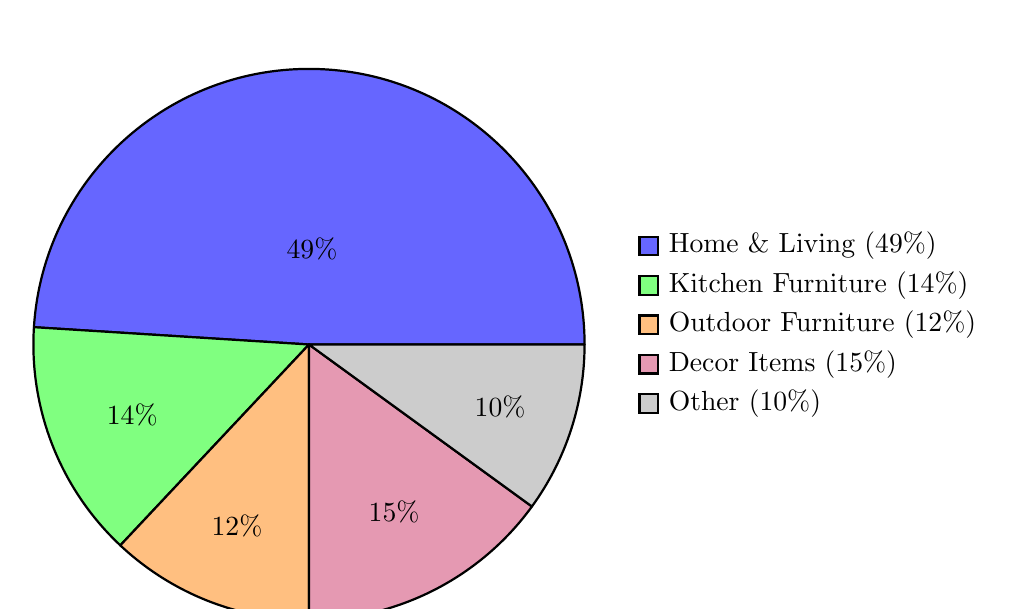
\begin{tikzpicture}
    \pie[
        text=legend,
        radius=3.5,
        color={blue!60, green!50, orange!50, purple!40, gray!40}
    ]{
        49/Home \& Living (49\%),
        14/Kitchen Furniture (14\%),
        12/Outdoor Furniture (12\%),
        15/Decor Items (15\%),
        10/Other (10\%)
    }
\end{tikzpicture}
\caption{Egyptian Furniture E-commerce Category Distribution by Revenue}
\label{fig:ecommerce_categories}
\end{figure}

Home \& Living dominates with 49\% revenue share, encompassing sofas, beds, wardrobes, and living room furniture, precisely the categories where visualization uncertainty drives cart abandonment. This category also exhibits the highest average order value (2,500-8,000 EGP) compared to Decor Items (200-600 EGP), maximizing affiliate commission potential for IntelliRoom's marketplace partnerships.

The data validates IntelliRoom's strategic focus on residential living spaces rather than commercial or outdoor applications: the combined Home \& Living plus Decor Items segments represent 64\% of total market value and directly align with the platform's room redesign core functionality.

\clearpage

% ============================================================================
\section{Competitive Landscape Analysis}
\label{sec:app_competitors}

The interior design technology market exhibits competitive intensity with both established players and emerging startups. However, comprehensive competitive analysis reveals that no existing platform combines AI-powered design generation with deep cultural intelligence for MENA markets, and this gap represents IntelliRoom's strategic positioning opportunity.

\subsection{Primary Competitors and Market Positioning}

\begin{table}[htbp]
\centering
\caption{Competitive Landscape Overview}
\label{tab:competitor_analysis}
\begin{tabular}{p{2cm}p{2.5cm}p{4.5cm}p{4cm}}
\toprule
\textbf{Platform} & \textbf{Target Segment} & \textbf{Core Strengths} & \textbf{Strategic Weaknesses} \\
\midrule
Coohom & Professionals & Arabic UI, 20K+ 3D models, established Egypt presence & Generic cultural features, no local marketplace, Western-focused design library \\
Planner 5D & DIY (90M users) & Massive user base, accessible interface, mobile-first & Basic AI capabilities, Western-centric aesthetics, limited professional features \\
Houzz Pro & Professionals & Comprehensive CRM, invoicing, business tools & Expensive (\$65/month), minimal AI design assistance, US-focused \\
IKEA Place & DIY & Best-in-class AR (98\% accuracy), completely free & Limited to IKEA catalog only, no design customization, Swedish aesthetics \\
\textbf{IntelliRoom} & Egypt/MENA & Cultural intelligence, gamification, local marketplace, affordable & New market entrant, building brand awareness \\
\bottomrule
\end{tabular}
\end{table}

\textbf{Coohom} represents the most direct competitive threat due to existing Egyptian market presence and Arabic interface. However, platform trials reveal that despite Arabic UI, the design output remains Western-focused: style recommendations emphasize Scandinavian minimalism, industrial lofts, and mid-century modern aesthetics with minimal understanding of Islamic geometric patterns, traditional Arabic furniture layouts, or Egyptian-specific spatial arrangements (e.g., sink placement near windows). Their 20,000+ model library contains fewer than 300 models representing traditional Middle Eastern furniture styles.

\textbf{Planner 5D's} 90 million user base demonstrates market validation for accessible 3D design tools. However, their AI capabilities remain rudimentary (basic room type detection without style intelligence), and user reviews consistently cite "doesn't understand my cultural preferences" as a pain point among MENA users. Their freemium model (free with limitations, \$10/month premium) establishes pricing expectations that IntelliRoom's strategy must consider.

\textbf{IKEA Place} provides strategic insights into AR furniture preview adoption: their 98\% object placement accuracy rate sets the technical benchmark users expect. However, their catalog limitation (IKEA products only) creates frustration for users seeking local furniture options, and IKEA's Scandinavian design language inherently conflicts with traditional Egyptian aesthetic preferences.

\subsection{Feature-by-Feature Competitive Analysis}

\begin{table}[htbp]
\centering
\caption{Detailed Feature Comparison Matrix}
\label{tab:feature_comparison}
\begin{tabular}{lcccc}
\toprule
\textbf{Feature Category} & \textbf{Coohom} & \textbf{Planner 5D} & \textbf{Houzz Pro} & \textbf{IntelliRoom} \\
\midrule
AI Design Intelligence & Yes & Limited & Limited & Advanced \\
3D Visualization Quality & Advanced & Good & Basic & Advanced \\
Arabic Language UI & Yes & No & No & Yes \\
Cultural Style Library & Limited & No & No & Deep \\
Local Marketplace Integration & No & No & No & Yes \\
Gamification \& Community & No & No & No & Yes \\
Custom Cultural LoRA Models & No & No & No & Yes \\
Free Tier Availability & Yes & Yes & No & Yes \\
Mobile-First Design & Partial & Yes & No & Yes \\
\bottomrule
\end{tabular}
\end{table}

The feature matrix reveals IntelliRoom's differentiation strategy: while competitors offer superior features in individual categories (Coohom's 3D quality, Planner 5D's mobile experience), none deliver the integrated value proposition of cultural intelligence + local marketplace + community engagement specifically optimized for Egyptian users.

\subsection{Strategic Gap Analysis}

Market gap analysis identifies four critical opportunity areas where existing solutions fail to meet MENA market needs:

\begin{table}[htbp]
\centering
\caption{Strategic Market Gap Analysis}
\label{tab:gap_analysis}
\begin{tabular}{p{2.5cm}p{4cm}p{4cm}p{3cm}}
\toprule
\textbf{Gap Category} & \textbf{Current Market State} & \textbf{IntelliRoom Solution} & \textbf{Defensibility} \\
\midrule
Cultural Depth & Arabic UI overlay on Western design engine & LoRA models trained on Egyptian/Islamic interior datasets, Ain Shams research partnership & Deep local expertise required \\
User Engagement & Passive AI processing (30-60s wait times) & Gamified voting during generation, community-driven model improvement & Novel approach \\
Local Commerce & External links to international retailers & Direct Egyptian retailer partnerships, local payment integration & Requires on-ground relationships \\
Professional Accessibility & Expensive tools (\$65+/month) or basic free tools & Powerful professional tier at accessible Egyptian pricing & Value positioning \\
\bottomrule
\end{tabular}
\end{table}

The \textbf{Cultural Depth} gap represents IntelliRoom's most defensible competitive advantage. Training custom LoRA models on Egyptian interior design datasets requires: (1) access to large volumes of culturally-relevant training images, (2) expertise in identifying authentic vs. tourist-focused design elements, (3) partnerships with Egyptian design institutes for validation, and (4) continuous refinement based on local user feedback. These requirements create substantial barriers to replication by international competitors lacking local presence and cultural knowledge.

The \textbf{User Engagement} gap addresses a universal pain point: AI generation requires 30-60 seconds processing time, during which users passively wait. IntelliRoom's gamification approach transforms this latency into engagement opportunity, allowing users to vote on design elements, participate in style preference surveys, and contribute to community model training, activities that simultaneously improve platform intelligence while reducing perceived wait times.

% ============================================================================
\section{Business Model and Revenue Strategy}
\label{sec:app_business_model}

IntelliRoom adopts a phased monetization strategy aligned with product-market fit validation timelines and graduation project constraints.

\subsection{Phase 1: Free Beta (Current Graduation Project Scope)}

The initial platform launch operates as a \textbf{Free Beta} accessible to all Egyptian users without payment requirements. This approach serves multiple strategic objectives: (1) maximizing user acquisition to demonstrate market traction, (2) gathering qualitative feedback to refine cultural design models, (3) validating technical architecture under real usage patterns, and (4) establishing initial Egyptian furniture retailer partnerships without revenue-sharing pressure.

During the beta phase, the platform implements "soft" monetization validation through tracking of key conversion indicators: furniture marketplace click-through rates, premium feature engagement metrics, and user feedback patterns. This data informs post-graduation pricing optimization without requiring actual payment infrastructure during the academic project phase.

\subsection{Phase 2: Freemium Monetization (Post-Graduation)}

Following successful product-market fit validation, IntelliRoom transitions to a freemium subscription model optimized for Egyptian purchasing power and payment preferences:

\begin{table}[htbp]
\centering
\caption{Planned Subscription Tier Structure (Post-Graduation Phase)}
\label{tab:subscription_tiers}
\begin{tabular}{p{2.5cm}p{2.5cm}p{2.5cm}p{5cm}}
\toprule
\textbf{Tier} & \textbf{Pricing} & \textbf{Target Segment} & \textbf{Key Features} \\
\midrule
Free & Permanent & User Acquisition & 3 designs/month, basic cultural styles, watermarked outputs, community gallery access \\
Premium & \textasciitilde199 EGP/month & Homeowners & Unlimited designs, all cultural styles, 4K resolution exports, no watermarks, AR preview (future) \\
Professional & \textasciitilde350 EGP/month & Interior Designers & All Premium features + team collaboration, client presentation mode, PDF export, project management tools \\
Business & Custom & Design Firms & Team accounts (5+ users), usage analytics, white-label options, API access, priority support \\
\bottomrule
\end{tabular}
\end{table}

Pricing strategy balances three factors: (1) Egyptian median household income (approximately 6,000 EGP/month), (2) competitive benchmarks (Planner 5D charges \$10/month = 500 EGP, Coohom charges \$29/month = 1,450 EGP), and (3) perceived value relative to traditional designer consultations (500-2,000 EGP per room). The Premium tier at 199 EGP represents approximately 3\% of median household income, positioning it as accessible for middle-class homeowners undertaking renovation projects.

The freemium model deliberately maintains accessible free tier limitations to enable users to complete typical single-room projects without payment, reducing conversion friction while creating upgrade incentives for users planning multi-room renovations or frequent design experimentation. Premium tiers offer significantly more generous limits and enhanced features.

\subsection{Marketplace Revenue Model}

Beyond subscription revenue, IntelliRoom captures value through affiliate partnerships with Egyptian furniture retailers and manufacturers. When users click "Shop This Look" or add recommended furniture to shopping carts, IntelliRoom earns commission on completed purchases (negotiated rates: 5-12\% depending on product category and order value).

Preliminary partnership discussions with Homzmart (Egypt's largest online furniture retailer) indicate willingness to offer 8\% commission on referrals, with higher rates (10-12\%) available for exclusive partnership arrangements. Given average furniture order values of 2,500-8,000 EGP, successful conversions generate 200-960 EGP per transaction, comparable to multiple months of Premium subscription revenue from a single marketplace transaction.

The marketplace model creates aligned incentives: retailers gain qualified traffic (users who have already visualized furniture in their spaces), users receive convenient purchasing options with local payment support, and IntelliRoom earns performance-based revenue without inventory or fulfillment risks.

% ============================================================================
\section{Risk Assessment and Mitigation Strategies}
\label{sec:app_risk_assessment}

Comprehensive risk analysis identifies five primary threat categories that could impact IntelliRoom's market success, along with corresponding mitigation strategies:

\begin{table}[htbp]
\centering
\caption{Strategic Risk Assessment Matrix}
\label{tab:risk_matrix}
\begin{tabular}{p{3cm}ccp{6cm}}
\toprule
\textbf{Risk Category} & \textbf{Probability} & \textbf{Impact} & \textbf{Mitigation Strategy} \\
\midrule
Competitive Response & High & High & Build defensible cultural expertise moat; unique gamification mechanics; establish exclusive local partnerships that global competitors cannot easily replicate \\
AI Quality Issues & Medium & High & Partner with Ain Shams University for academic validation; curate high-quality training datasets; implement continuous user feedback loops for model refinement \\
User Acquisition Costs & Medium & High & Leverage team's marketing expertise; establish university campus partnerships; deploy viral social media strategy; utilize community-driven growth \\
Infrastructure Costs & Medium & Medium & Employ pay-per-use AI APIs; implement generation limits on free tier; continuously optimize model efficiency to reduce per-request costs \\
Payment Integration & Low & Medium & Partner with established Egyptian payment providers (Fawry, InstaPay); support local payment methods through marketplace partners \\
\bottomrule
\end{tabular}
\end{table}

\textbf{Competitive Response Risk} (High probability, High impact): If IntelliRoom demonstrates market traction, well-funded competitors (particularly Coohom with existing Egyptian presence) may rapidly add Egyptian cultural design features. Mitigation requires building defensible advantages through: (1) exclusive partnerships with Egyptian furniture manufacturers offering special pricing unavailable to international platforms, (2) continuous refinement of cultural design models through local user feedback loops that competitors cannot easily replicate, and (3) community network effects where users generate cultural design content that improves platform intelligence.

\textbf{AI Quality Issues} (Medium probability, High impact): Users expect photorealistic outputs that respect structural constraints (walls, windows remain intact) while applying cultural styles authentically. Poor quality outputs drive immediate abandonment. Mitigation strategies include rigorous testing with diverse room types, partnership with Ain Shams University design faculty for qualitative validation, and transparent "beta" labeling that manages expectations during quality refinement phases.

\textbf{User Acquisition Costs} (Medium probability, High impact): Customer acquisition cost (CAC) in Egyptian digital markets averages 50-150 EGP per user through paid channels, creating unsustainable economics given free beta positioning. Mitigation emphasizes zero-cost acquisition channels: viral social media campaigns showcasing before/after transformations, university partnerships leveraging team members' ASU networks, and referral programs offering credit rewards for successful friend invitations.

% ============================================================================
\section{Success Metrics and Validation Framework}
\label{sec:app_success_metrics}

The beta phase validation framework establishes quantitative and qualitative success criteria across three evaluation timeframes:

\begin{table}[htbp]
\centering
\caption{Beta Phase Validation Milestones and Success Criteria}
\label{tab:milestones}
\begin{tabular}{lp{10cm}}
\toprule
\textbf{Timeline Phase} & \textbf{Success Criteria and Key Metrics} \\
\midrule
3-Month Initial Validation & 500-1,000 registered users, positive qualitative feedback on cultural authenticity (NPS >30), establishment of 2-3 Egyptian furniture retailer partnerships, technical infrastructure stability (<5\% error rate) \\
6-Month Product-Market Fit & 2,000-5,000 active users, demonstrated user retention (>40\% 7-day retention, >20\% 30-day retention), feature usage validation (>60\% users try AI redesign, >30\% explore marketplace), generation quality satisfaction (>70\% positive ratings) \\
12-Month Scale Readiness & 10,000-20,000 total users, proven viral growth coefficient (k >0.5), demonstrated premium feature interest through user engagement patterns, marketplace conversion tracking (>5\% click-to-purchase rate), technical readiness for monetization phase \\
\bottomrule
\end{tabular}
\end{table}

\textbf{Critical Success Indicators:} Beyond raw user counts, product-market fit validation emphasizes qualitative metrics indicating cultural resonance: user testimonials explicitly mentioning "Egyptian style" or "matches my culture," designer testimonials validating time savings, and organic social media sharing of generated designs without platform prompting (indicating genuine user satisfaction rather than incentivized behavior).

\textbf{Failure Indicators and Pivot Triggers:} If 6-month metrics fall significantly below targets (<1,000 active users, <20\% 7-day retention, <50\% design satisfaction), the project roadmap includes defined pivot options: (1) narrow focus to professional designer segment only, (2) expand culturally-neutral feature set to validate technical capabilities before adding cultural intelligence, or (3) pivot to B2B model serving furniture retailers directly rather than consumer-facing platform.

% ============================================================================
\section{Strategic Recommendations and Conclusions}
\label{sec:app_conclusions}

This comprehensive market analysis validates substantial opportunity for AI-powered interior design platforms serving MENA markets, with Egypt representing the optimal launch geography. Key strategic conclusions inform IntelliRoom's development roadmap:

\textbf{Conclusion 1: Cultural Intelligence Represents Defensible Differentiation.} Competitive analysis confirms no existing platform delivers sophisticated cultural design intelligence for Egyptian/MENA markets despite clear demand indicators. This gap creates first-mover advantage opportunity, provided IntelliRoom executes superior cultural training data curation and maintains continuous quality refinement through local user feedback.

\textbf{Conclusion 2: Freemium-to-Marketplace Revenue Model Aligns with Egyptian Economics.} Direct subscription revenue faces headwinds from Egyptian purchasing power constraints and payment infrastructure limitations. The hybrid model (generous free tier for user acquisition, marketplace affiliate revenue for monetization) better aligns with local market dynamics while deferring payment friction until users demonstrate high purchase intent.

\textbf{Conclusion 3: Launch Timing Critical for Seasonal Capture.} February-March 2026 launch positioning enables capture of April peak renovation demand (Ramadan/Eid preparation), the single highest-value acquisition window representing 15-20\% of annual market activity. Delayed launch missing this window would sacrifice 3-4 months of optimal user acquisition conditions.

\textbf{Conclusion 4: Community and Gamification Enhance Competitive Moat.} Network effects created through community design sharing and gamified model training create switching costs and data advantages that pure-technology competitors cannot easily replicate. Prioritizing these features in initial launch (rather than deferring to "future enhancements") strengthens defensibility from day one.

\textbf{Recommended Strategic Actions:} (1) Accelerate LoRA model training for Egyptian cultural styles to achieve launch-ready quality by February 2026, (2) finalize minimum 2 furniture retailer partnerships pre-launch to enable marketplace functionality from day one, (3) establish Ain Shams University design faculty advisory relationship for ongoing cultural validation, (4) develop viral social media content strategy showcasing authentic Egyptian interior transformations to drive zero-cost user acquisition.


% ============================================================================
% Appendix B: Use Case Documentation
% ============================================================================

\chapter{Use Case Documentation}
\label{app:use_cases}

This appendix documents the core use cases for the IntelliRoom AI platform, focusing on the three primary user workflows that define the platform's value proposition: AI-powered design generation, intelligent room analysis, and integrated furniture shopping.

% ============================================================================
\section{Overview}
\label{sec:app_uc_overview}

IntelliRoom serves three primary user groups: homeowners seeking affordable design solutions, professionals requiring efficient client presentation tools, and furniture retailers connecting with motivated buyers. The platform's core functionality revolves around AI-powered room transformation with integrated marketplace features.

% ============================================================================
\section{Use Case Diagram}
\label{sec:app_uc_diagram}

\begin{figure}[htbp]
    \centering
    \includegraphics[width=1.0\textwidth]{figures/UC_Professional.png}
    \caption{Professional Designer Workflows}
    \label{fig:uc_professional}
\end{figure}

\begin{figure}[htbp]
    \centering
    \includegraphics[width=1.0\textwidth]{figures/UC_Admin.png}
    \caption{Administrator and System Management Workflows}
    \label{fig:uc_admin}
\end{figure}

% ============================================================================
\section{Core Use Case Specifications}
\label{sec:app_core_uc}

This section provides detailed specifications for the three most critical use cases that define IntelliRoom's core value proposition.

% ----------------------------------------------------------------------------
\subsection{UC-C04: Upload \& Analyze Room}
\label{sec:uc_upload_analyze}

\begin{table}[h]
\centering
\caption{UC-C04: Upload \& Analyze Room Photo - Detailed Specification}
\label{tab:uc_upload_detail}
\begin{tabular}{p{3cm}p{11cm}}
\toprule
\textbf{Attribute} & \textbf{Description} \\
\midrule
Use Case ID & UC-C04 \\
\midrule
Name & Upload \& Analyze Room Photo \\
\midrule
Actors & Consumer/Professional User, AI Analysis System (Florence-2, SAM2) \\
\midrule
Preconditions & User authenticated, navigated to design workflow, AI pipeline operational \\
\midrule
Basic Flow &
\begin{enumerate}[leftmargin=*,noitemsep,topsep=0pt]
    \item User uploads image or captures photo
    \item System validates and uploads to backend storage
    \item \textbf{Florence-2} analyzes: room type, furniture items, architectural features, lighting
    \item \textbf{SAM2} generates: pixel-level masks (walls/floors/furniture), depth map, replacement regions
    \item System stores metadata in MongoDB and displays preview
    \item User confirms or requests re-analysis, then proceeds to style selection
\end{enumerate} \\
\midrule
Alternative Flows &
\begin{itemize}[leftmargin=*,noitemsep,topsep=0pt]
    \item A1: Invalid format/low quality - System prompts correction
    \item A2: Detection failure - Manual room type selection offered
    \item A3: Timeout (>30s) - Retry or manual selection
\end{itemize} \\
\midrule
Postconditions & Image and Florence-2 metadata stored; SAM2 masks saved for ControlNet; style selection enabled \\
\midrule
Includes & None \\
\midrule
Extends & UC-C05 (Choose Style), UC-C06 (Generate AI Design) \\
\midrule
Technical Notes & 
Florence-2 runs on ComfyUI backend or via Replicate API. SAM2 segmentation provides structural guidance for ControlNet to preserve room geometry during style transfer. Analysis typically completes in 5-10 seconds. \\
\bottomrule
\end{tabular}
\end{table}

\clearpage

% ----------------------------------------------------------------------------
\subsection{UC-C06: Generate AI Design}
\label{sec:uc_generate_design}

\begin{table}[h]
\centering
\caption{UC-C06: Generate AI Design - Detailed Specification}
\label{tab:uc_generate_detail}
\begin{tabular}{p{3cm}p{11cm}}
\toprule
\textbf{Attribute} & \textbf{Description} \\
\midrule
Use Case ID & UC-C06 \\
\midrule
Name & Generate AI Design \\
\midrule
Actors & Consumer/Professional User, AI Generation System (ComfyUI, ControlNet, LoRA Models) \\
\midrule
Preconditions & User authenticated, room analyzed (UC-C04), style selected (UC-C05), generation quota available, ComfyUI operational \\
\midrule
Basic Flow &
\begin{enumerate}[leftmargin=*,noitemsep,topsep=0pt]
    \item User confirms parameters; system validates quota
    \item ComfyUI pipeline executes 4 stages:
    \begin{itemize}[noitemsep,topsep=0pt]
        \item \textbf{ControlNet:} Preserves structure using SAM2 masks
        \item \textbf{LoRA:} Applies Egyptian/Islamic/Modern styles
        \item \textbf{Stable Diffusion:} Refines textures and lighting
        \item \textbf{Post-processing:} Validates cultural authenticity
    \end{itemize}
    \item During processing, user votes on design pairs, earns credits
    \item System stores design with metadata, presents before/after comparison
    \item User can view variations, save, download, or regenerate
\end{enumerate} \\
\midrule
Alternative Flows &
\begin{itemize}[leftmargin=*,noitemsep,topsep=0pt]
    \item A1: Quota exhausted - Upgrade prompt
    \item A2: Timeout (>120s) - Retry or email notification
    \item A3: Low quality - Auto-regeneration
\end{itemize} \\
\midrule
Postconditions & Design stored with unique ID, quota decremented (free tier), added to gallery, voting data sent for training \\
\midrule
Includes & UC-C10 (Gamified Voting During Generation), UC-C14 (View Free Tier Limits) \\
\midrule
Extends & UC-C15 (Purchase Premium) for 4K resolution, UC-C07 (View Variations) for unlimited options \\
\midrule
Technical Notes & 
ControlNet ensures structural fidelity by using depth/edge maps from SAM2. \\
\bottomrule
\end{tabular}
\end{table}

\clearpage

% ----------------------------------------------------------------------------
\subsection{UC-M02: Shop This Look}
\label{sec:uc_shop_this_look}

\begin{table}[h]
\centering
\caption{UC-M02: Shop This Look - Detailed Specification}
\label{tab:uc_shop_detail}
\begin{tabular}{p{3cm}p{11cm}}
\toprule
\textbf{Attribute} & \textbf{Description} \\
\midrule
Use Case ID & UC-M02 \\
\midrule
Name & Shop This Look (AI-Powered Furniture Matching) \\
\midrule
Actors & Consumer User, Product Matching System (Florence-2, CLIP), Egyptian Furniture Retailers \\
\midrule
Preconditions & User has generated design (UC-C06), clicks "Shop This Look", retailer catalog populated \\
\midrule
Basic Flow &
\begin{enumerate}[leftmargin=*,noitemsep,topsep=0pt]
    \item \textbf{Florence-2} detects furniture items and extracts visual features
    \item \textbf{CLIP} matches items to Egyptian retailer products
    \item System displays interactive overlay with clickable hotspots
    \item Side panel shows 3-5 products per item: name, price (EGP), retailer, similarity, stock
    \item User clicks hotspot to view full details: specs, images, reviews, alternatives
    \item User adds items to cart (UC-M08); system tracks conversion for analytics
\end{enumerate} \\
\midrule
Alternative Flows &
\begin{itemize}[leftmargin=*,noitemsep,topsep=0pt]
    \item A1: No matches or low confidence (<0.6) - Manual browsing or category suggestions
    \item A2: Out of stock - Notify option and alternatives
    \item A3: User filters - Re-run matching with constraints
\end{itemize} \\
\midrule
Postconditions & Products linked to design, cart updated, analytics logged, affiliate tracking attached \\
\midrule
Includes & UC-M01 (Browse Egyptian Furniture Catalog) for product data access \\
\midrule
Extends & UC-M05 (Compare Prices), UC-M08 (Add to Cart), UC-M10 (Place Order) \\
\midrule
Technical Notes & 
Florence-2 provides object detection, while CLIP enables semantic similarity matching. \\
\bottomrule
\end{tabular}
\end{table}

\clearpage

% ============================================================================
\section{Supporting Use Case Summary}
\label{sec:app_supporting_uc}

The following table summarizes additional use cases that support the platform's complete functionality. Detailed specifications are available in the requirements documentation.

\begin{longtable}{p{3.5cm}p{10cm}}
\caption{Supporting Use Cases Summary} \label{tab:supporting_uc} \\
\toprule
\textbf{Use Case ID} & \textbf{Description} \\
\midrule
\endfirsthead
\toprule
\textbf{Use Case ID} & \textbf{Description} \\
\midrule
\endhead
\midrule
\endfoot
\bottomrule
\endlastfoot

\multicolumn{2}{c}{\textbf{Consumer Account \& Access}} \\
\midrule
UC-C01: Register Account & User creates account with email, password, profile information. Email verification required. \\
UC-C02: Log In / Log Out & User authenticates with credentials to access personalized features. Session management. \\
UC-C03: Manage Profile & User updates personal information, design preferences, notification settings. \\
\midrule

\multicolumn{2}{c}{\textbf{Consumer Design Workflow}} \\
\midrule
UC-C05: Choose Style/Theme & User selects cultural design style (Egyptian, Islamic, Modern, Mediterranean) before generation. \\
UC-C07: View Design Variations & User reviews multiple design options with before/after comparison slider. \\
UC-C08: Save/Favorite Design & User saves generated designs to personal gallery for later access. \\
UC-C09: Download Design Image & User downloads design in available resolution (1080p free, 4K premium). Watermark on free tier. \\
\midrule

\multicolumn{2}{c}{\textbf{Consumer Engagement}} \\
\midrule
UC-C10: Gamified Voting & User ranks design pairs during AI generation (30-60s), contributes to model improvement. \\
UC-C11: Earn Credits & User earns credits through voting, sharing, daily streaks. Credits unlock premium features. \\
UC-C12: Browse Community Gallery & User explores designs shared by other users, filtered by style and room type. \\
UC-C13: Share to Social Media & User shares designs to Facebook, Instagram, WhatsApp with customizable templates. \\
\midrule

\multicolumn{2}{c}{\textbf{Marketplace Shopping}} \\
\midrule
UC-M01: Browse Furniture Catalog & User explores curated Egyptian furniture catalog organized by category and style. \\
UC-M03: Filter by Style/Culture & User filters products by Egyptian, Islamic, Modern themes matching design generation styles. \\
UC-M05: Compare Prices & User compares pricing for similar items across multiple Egyptian retailers side-by-side. \\
UC-M08: Add to Cart & User adds products to shopping cart. Cart persists across sessions. \\
UC-M09: Select Payment Method & User selects credit card, Fawry, or InstaPay mobile payment. \\
UC-M10: Place Order & User confirms order. Order routed to retailer for fulfillment with tracking. \\
\midrule

\multicolumn{2}{c}{\textbf{Professional Designer Tools}} \\
\midrule
UC-P01: Register Professional Account & Designer creates professional account with portfolio, credentials, business information. \\
UC-P04: Create Client Project & Designer creates project with client information, requirements, timeline. Multi-room support. \\
UC-P08: Priority Queue Generation & Professional users get priority AI processing for faster client turnaround. \\
UC-P10: Batch Process Rooms & Designer processes multiple rooms simultaneously for commercial projects (cafes, offices). \\
UC-P17: Share Client Preview Link & Designer generates read-only link for client to view designs without account. \\
UC-P20: Export PDF Report & Designer generates branded PDF with before/after comparisons and shopping lists. \\

\end{longtable}


% ============================================================================
% Appendix C: Business Model Canvas
% ============================================================================

\chapter{Business Model Canvas}
\label{app:business_model}

This appendix presents the Business Model Canvas for IntelliRoom, providing a strategic view of the platform's value creation, delivery, and monetization approach.

% ============================================================================
\section{Business Model Overview}
\label{sec:app_bmc_visual}

The IntelliRoom Business Model Canvas captures the key elements of our business strategy for the Egyptian and MENA interior design market.

\subsection{Key Partners}

\begin{itemize}
    \item Egyptian furniture manufacturers (Mobica, Divano, Danube Home)
    \item Payment gateways (Fawry, InstaPay, PayMob)
    \item Cloud providers (Vercel, Railway, Supabase)
    \item AI model communities and APIs (Replicate, RunPod)
    \item Interior design influencers
    \item Ain Shams University architectural engineering department
\end{itemize}

\subsection{Key Activities}

\begin{itemize}
    \item AI model training with custom LoRA for Egyptian/Islamic styles
    \item Platform development and maintenance
    \item Retailer partnership onboarding and management
    \item Cultural content curation with architectural partners
    \item Community management and moderation
    \item Marketing and user acquisition campaigns
\end{itemize}

\subsection{Key Resources}

\begin{itemize}
    \item AI infrastructure (SAM2, ControlNet, Florence-2, ComfyUI)
    \item Egyptian furniture catalog database
    \item Culturally-authentic design training datasets
    \item Cross-disciplinary development team
    \item GPU compute resources (pay-per-use APIs)
    \item University partnership network
\end{itemize}

\subsection{Value Propositions}

\begin{itemize}
    \item Culturally-aware AI design for Egyptian/MENA aesthetics
    \item Integrated Egyptian furniture marketplace
    \item Affordable alternative to traditional professional design services
    \item Full Arabic language support
    \item Local payment methods (Fawry, InstaPay)
    \item Community inspiration gallery
    \item Gamified engagement during AI processing
\end{itemize}

\subsection{Customer Relationships}

\begin{itemize}
    \item Self-service platform with intuitive UX
    \item Tutorial content and onboarding
    \item WhatsApp Business support
    \item Community forums and galleries
    \item Email notifications and engagement
    \item Gamified loyalty program (credits, streaks)
\end{itemize}

\subsection{Customer Segments}

\begin{itemize}
    \item Egyptian homeowners (45\% of target market)
    \item Young professionals (25-34 age group)
    \item Families renovating homes
    \item Interior design professionals (43\% of target market)
    \item Small businesses (cafes, offices, clinics) (12\% of target market)
    \item Real estate agents and property developers
\end{itemize}

\subsection{Channels}

\begin{itemize}
    \item Web Application (PWA for mobile-first experience)
    \item Social Media (Instagram, TikTok, Facebook)
    \item WhatsApp Business for support and marketing
    \item Egyptian furniture retailer partnerships
    \item Influencer marketing collaborations
    \item University and architecture school partnerships
\end{itemize}

\subsection{Revenue Streams}

\textbf{Initial Launch Phase - Free Beta:}

The IntelliRoom platform will launch as a \textbf{completely free beta} for all users during the initial deployment phase (estimated 6-12 months post-graduation). This allows the team to:
\begin{itemize}
    \item Validate product-market fit with real Egyptian users
    \item Collect user feedback for feature refinement
    \item Build brand awareness and user base
    \item Establish retailer partnerships and marketplace operations
    \item Train and optimize AI models with real-world usage data
\end{itemize}

\textbf{Future Phase - Monetization Strategy:}

Following successful beta validation, IntelliRoom will transition to a freemium subscription model:
\begin{itemize}
    \item \textbf{Free Tier:} Limited AI generations per month, basic styles, watermarked downloads (continues indefinitely for user acquisition)
    \item \textbf{Premium Tier:} Significantly more generous generation limits, full Egyptian/Islamic style library, 4K downloads, no watermarks
    \item \textbf{Professional Tier:} Unlimited generations plus collaboration tools, client presentation features, priority queue, PDF exports
    \item \textbf{Business Tier:} To be determined based on enterprise needs, featuring team accounts, analytics, white-label options
    \item \textbf{Marketplace Revenue:} Affiliate commissions on furniture sales referred to Egyptian retailers (percentage-based, negotiated per partner)
    \item \textbf{Future Opportunities:} Featured retailer placements, B2B API access, white-label partnerships with real estate developers
\end{itemize}

The pricing strategy emphasizes affordability for the Egyptian market while remaining sustainable. All pricing remains flexible and subject to adjustment based on beta phase learnings and market conditions.

% ============================================================================
\section{Detailed Component Analysis}
\label{sec:app_bmc_detail}

\subsection{Value Proposition Summary}

IntelliRoom's core value centers on democratizing culturally-aware interior design for MENA markets through: (1) cultural intelligence understanding Egyptian/Islamic aesthetics, (2) local furniture marketplace integration with EGP pricing, (3) accessibility for middle-class families, (4) Arabic language and local payment support, and (5) community-driven inspiration.

\subsection{Customer Segments}

\begin{table}[h]
\centering
\caption{Target Customer Segments}
\begin{tabular}{p{3.5cm}p{3cm}p{5cm}}
\toprule
\textbf{Segment} & \textbf{Share} & \textbf{Key Needs} \\
\midrule
Young Professionals (25-35) & Primary & Affordable first-home design, social sharing \\
Egyptian Families (35-50) & Secondary & Renovation visualization, purchase confidence \\
Design Professionals & 43\% & Client presentation, rapid visualization \\
Small Businesses & 12\% & Commercial space design on budget \\
\bottomrule
\end{tabular}
\end{table}

% ============================================================================
\section{Growth Strategy}
\label{sec:app_growth}

\begin{table}[h]
\centering
\caption{Growth Phase Summary}
\begin{tabular}{p{3cm}p{3cm}p{6.5cm}}
\toprule
\textbf{Phase} & \textbf{Timeline} & \textbf{Key Objectives} \\
\midrule
Free Beta & Months 1-6 & 1,000-5,000 users, 2-3 retailer partnerships, product-market fit \\
Beta Scaling & Months 7-12 & 10,000-50,000 users, marketplace validation, prepare monetization \\
Monetization & Months 12-24 & Paid tiers, sustainable revenue, GCC expansion exploration \\
\bottomrule
\end{tabular}
\end{table}

% ============================================================================
\section{Competitive Advantages}
\label{sec:app_competitive}

IntelliRoom's sustainable competitive advantages include: (1) \textbf{Cultural Moat} requiring authentic local expertise, (2) \textbf{Network Effects} from community-driven AI improvement, (3) \textbf{Local Partnerships} with Egyptian retailers and universities, and (4) \textbf{First-Mover} positioning in the underserved MENA market.

% ============================================================================
\section{Risk Mitigation}
\label{sec:app_risk}

\subsection{Key Risks and Mitigation Strategies}

\begin{table}[h]
\centering
\caption{Risk Mitigation Matrix}
\label{tab:risk_mitigation}
\begin{tabular}{p{3cm}p{5cm}p{5cm}}
\toprule
\textbf{Risk} & \textbf{Impact} & \textbf{Mitigation} \\
\midrule
Competitive Response & Global players add cultural features & Deepen local partnerships, accelerate innovation, leverage network effects \\
\midrule
User Acquisition & High acquisition costs in competitive market & Leverage team marketing expertise, viral features, referral program \\
\midrule
AI Quality Issues & Cultural authenticity failures & Ain Shams partnership validation, user feedback loops, expert curation \\
\midrule
Infrastructure Costs & Compute costs during free beta & Pay-per-use model, generation limits, efficiency optimization \\
\midrule
Currency Volatility & Egyptian Pound depreciation & Flexible EGP-based pricing, gradual localization, USD reserves \\
\bottomrule
\end{tabular}
\end{table}


% ============================================================================
% Appendix D: Additional UI Mockups
% ============================================================================

\chapter{Additional User Interface Mockups}
\label{app:ui_mockups}

This appendix provides additional user interface mockups beyond the core screens presented in Chapter~\ref{chap:design}. These designs cover authentication flows and subscription management.

% ============================================================================
\section{Authentication Screens}
\label{sec:app_ui_auth}

\subsection{Login Screen}

The login screen (Figure~\ref{fig:app_ui_login}) provides returning users with secure access to their accounts. The interface emphasizes ease of use with social authentication options and traditional email/password login.

\begin{figure}[htbp]
    \centering
    \includegraphics[width=0.8\textwidth]{figures/ui/auth_login.png}
    \caption{Login Interface: Secure user authentication with social login integration (Google, Facebook).}
    \label{fig:app_ui_login}
\end{figure}

Design considerations for the login screen:
\begin{itemize}
    \item Clean, minimalist design with centered modal layout
    \item Social login buttons prominently displayed above traditional form
    \item Clear visual hierarchy with ``Welcome Back'' header
    \item Direct link to registration for new users
    \item Mobile-responsive layout with touch-friendly input fields
\end{itemize}

\subsection{Registration Screen}

The registration screen (Figure~\ref{fig:app_ui_register}) guides new users through account creation with comprehensive input validation and social registration options.

\begin{figure}[htbp]
    \centering
    \includegraphics[width=0.8\textwidth]{figures/ui/auth_signup.png}
    \caption{Registration Interface: Comprehensive sign-up form collecting user profile data with social registration alternatives.}
    \label{fig:app_ui_register}
\end{figure}

Key features of the registration screen:
\begin{itemize}
    \item Structured form collecting first name, last name, email, username, and password
    \item Password confirmation field with visual feedback
    \item Social registration options (Google, Facebook) for streamlined onboarding
    \item ``Become an artist!'' value proposition encouraging content creation
    \item Direct link to login page for returning users
    \item Mobile-responsive centered modal layout
\end{itemize}

% ============================================================================
\section{Pricing and Subscription}
\label{sec:app_ui_payment}

\subsection{Pricing Plans Screen}

The pricing page (Figure~\ref{fig:app_ui_pricing}) displays available subscription tiers with clear feature comparison, guiding users in selecting the appropriate plan for their needs.

\begin{figure}[htbp]
    \centering
    \includegraphics[width=1.0\textwidth]{figures/ui/pricing_plans.png}
    \caption{Pricing \& Plans Interface: Comparison of subscription tiers (Free, Pro, Business) with feature breakdowns and monthly/annual toggle.}
    \label{fig:app_ui_pricing}
\end{figure}

Key features of the pricing interface:
\begin{itemize}
    \item Three-tier pricing structure: Free, Pro (\$29/month), Business (\$99/month)
    \item Monthly/Annual billing toggle with 17\% savings indicator
    \item Feature comparison highlighting limitations and capabilities
    \item ``Most Popular'' badge on the Pro tier guiding user selection
    \item Clear call-to-action buttons for each tier
    \item Transparent feature listing including design limits, resolution options, style library access, and support levels
\end{itemize}

This interface satisfies requirements FR-30 (subscription management) and NFR-06 (transparent pricing).

% ============================================================================
\section{Responsive Design Considerations}
\label{sec:app_ui_responsive}

All interface screens are designed to be responsive across device sizes:

\begin{table}[htbp]
    \centering
    \caption{Responsive Breakpoints}
    \label{tab:app_breakpoints}
    \begin{tabular}{|l|l|l|}
        \hline
        \textbf{Device} & \textbf{Breakpoint} & \textbf{Layout Adaptation} \\
        \hline
        Mobile (Portrait) & 320px -- 480px & Single column, bottom navigation \\
        \hline
        Mobile (Landscape) & 481px -- 767px & Single column, expanded controls \\
        \hline
        Tablet & 768px -- 1024px & Two column, sidebar navigation \\
        \hline
        Desktop & 1025px -- 1440px & Full layout, sidebar + content \\
        \hline
        Large Desktop & 1441px+ & Full layout with max-width container \\
        \hline
    \end{tabular}
\end{table}

Key responsive design principles:
\begin{itemize}
    \item Touch-friendly targets (minimum 44px × 44px)
    \item Mobile-first CSS approach
    \item Progressive enhancement for larger screens
    \item Lazy loading for gallery images
    \item Optimized image delivery based on viewport
\end{itemize}

% ============================================================================
\section{Accessibility Considerations}
\label{sec:app_ui_a11y}

All interfaces adhere to WCAG 2.1 AA standards (NFR-11):

\begin{itemize}
    \item Color contrast ratios minimum 4.5:1 for text
    \item Keyboard navigation support throughout
    \item ARIA labels for interactive elements
    \item Focus indicators for all interactive elements
    \item Screen reader compatible structure
    \item Reduced motion options for animations
\end{itemize}

\vspace{1cm}
\textit{This appendix provides additional UI mockups. For core interface designs including Dashboard, Design Workspace, Marketplace, and Floor Planner, see Chapter~\ref{chap:design}.}


\end{appendices}

\end{document}
